\section{Numerische L"osung\label{section:lorenz2:numeric-solution}}
\rhead{Numerische L"osung}
Mit den \cref{equation:lorenz2:dota,equation:lorenz2:dotb} aus 
\cref{section:lorenz2:ho-model} haben wir Gleichungen gefunden, die wir mit 
Hilfe eines Computers berechnen k"onnen. Wobei wir dabei nat"urlich 
unterschiedlich vorgehen k"onnen. Was wir sicher brauchen, ist ein Programm, 
mit dessen Hilfe wir gew"ohnliche Differentialgleichungen l"osen k"onnen. In 
unserem Fall traf die Wahl auf \texttt{octave}, nicht nur weil es auf allen 
g"angigen Plattformen verf"ugbar und open-source ist, sondern weil es mit 
\texttt{lsode} einen m"achtigen  ODE-Solver beinhaltet.

Wie sich herausstellt, ist eine direkte Implementation unserer gefundenen 
gew"ohnlichen Differentialgleichungen \cref{equation:lorenz2:dota} und 
\cref{equation:lorenz2:dotb} in \texttt{octave} keine sonderlich effiziente 
L"osung, da der Algorithmus selbst f"ur kleine Grad $k$, auf dem Testsystem mit 
einer Intel\textregistered Core\texttrademark\, i7-3930K CPU mit 3.20 GHz, sehr 
lange dauert.

Um das ganze etwas zu optimieren, nehmen wir also am besten ein 
Computer-Algebra Programm, mit dessen die Gleichungen bereits soweit 
vereinfachen k"onnen, dass nur noch ein Vektor mit einfachen Summen "ubrig 
bleibt. Mit \texttt{maxima} haben wir dazu wieder ein open-source Programm das 
auf allen Plattformen zur Verf"ugung steht.

Wir haben jetzt alles zusammen um die Gleichungen mit \texttt{maxima} zu 
vereinfachen und uns eine Funktion f"ur \texttt{octave} zu generieren, die 
schnell ist. Trotz unseren Optimierungen ist das L"osen der 
Gleichungen immer noch "ausserst Rechen- und Zeitintensiv. Dies zeigen auch 
Laufzeitmessungen f"ur das Zeitintervall $t = [0,100]$ und f"ur $t = [0,40]$ 
auf dem Testsystem, die in \cref{figure:lorenz2:timings} veranschaulicht sind. 
Die Laufzeit liegt gem"ass diesen Messungen etwa bei $\text{O}(k^5)$ mit einer 
Tendenz zu sogar $\text{O}(k^6)$.

Eine der Ursachen f"ur die stark wachsende Laufzeit kann die fehlende 
Parallelisierung des Algorithmus sein, was dazu f"uhrt, dass f"ur jeden Grad 
$k$ nur ein CPU Core verwendet wird. Das erlaubt es uns zwar die Berechnung 
einzelner Grade $k$ gleichzeitig durchzuf"uhren, indem wir unterschiedliche 
\texttt{octave}-Instanzen f"ur die jeweiligen $k$ starten, doch ist der Nutzen 
aufgrund der rasant wachsenden Laufzeit nicht sonderlich gross. Zudem hat auch 
die Wahl des $t$-Intervalls und auch die an \texttt{lsode} gestellten 
Toleranzen Auswirkungen auf die Laufzeit. So kann man durch Lockerung unserer 
absoluten und relativen Toleranzabweichung von $10^{-12}$ respektive $10^{-13}$ 
mit Sicherheit noch etwas an Laufzeit gewinnen, was dann aber zu einem Verlust 
an Genauigkeit f"uhren w"urde.

Noch gar nicht angesprochen wurden die gew"ahlten Anfangsbedingungen und 
Parameterwerte. Bei den Anfangswerten setzen wir alles bis auf $b_{(0,2)}$ und 
$b_{(1,1)}$ gleich $0$, dies da diese Bereits f"ur Grad $2$ Verf"ugbar sind. 
Die Parameter sind so gew"ahlt, dass sie chaotisches Verhalten f"ur ein 
dreidimensionales Lorenzsystem, also eines mit Grad $2$, hervorrufen. 
Experimentell konnten so die Werte
\begin{align*}
	a = \sqrt{1/2},
	\qquad T_0 = 5,
	\qquad c = 82,
	\qquad \nu = 1.43,
	\qquad \text{und}
	\qquad \kappa = 0.143
\end{align*}
bestimmt werden.

Mit all dem sind die Lorenzsysteme mit Grad $k = \{2,3,\dots,22\}$ erfolgreich 
berechnet worden. Das hat teilweise zu erstaunlichen Ergebnissen gef"uhrt, wie 
\cref{figure:lorenz2:systemdeg2,figure:lorenz2:systemdeg3,figure:lorenz2:systemdeg4,figure:lorenz2:systemdeg5,figure:lorenz2:systemdeg6,figure:lorenz2:systemdeg7,figure:lorenz2:systemdeg8,figure:lorenz2:systemdeg9,figure:lorenz2:systemdeg10,figure:lorenz2:systemdeg11,figure:lorenz2:systemdeg12,figure:lorenz2:systemdeg13,figure:lorenz2:systemdeg14,figure:lorenz2:systemdeg15,figure:lorenz2:systemdeg16,figure:lorenz2:systemdeg17,figure:lorenz2:systemdeg18,figure:lorenz2:systemdeg19,figure:lorenz2:systemdeg20,figure:lorenz2:systemdeg21-40,figure:lorenz2:systemdeg22-40}
zeigen. Eines der augenf"alligsten ist, das ab $k = 4$ das chaotische Verhalten 
verschwindet. Das kann einerseits an unsere Reduktion des Ursprungssystems 
liegen oder der fehlenden Untersuchung des Anfangsbedingungs- und 
Parameterraumes.

\begin{figure}
	\centering
	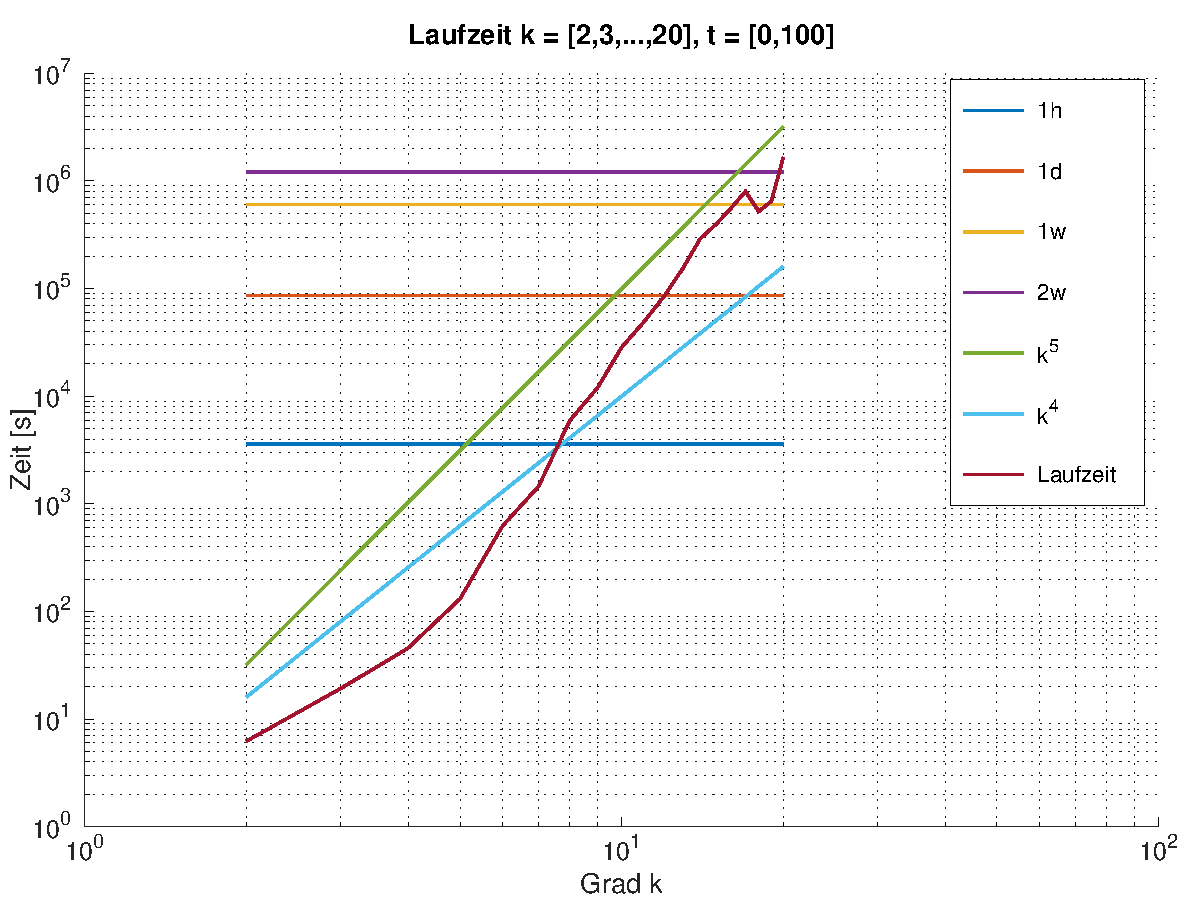
\includegraphics[width=0.49\linewidth]{lorenz2/03-images/timing_100}
	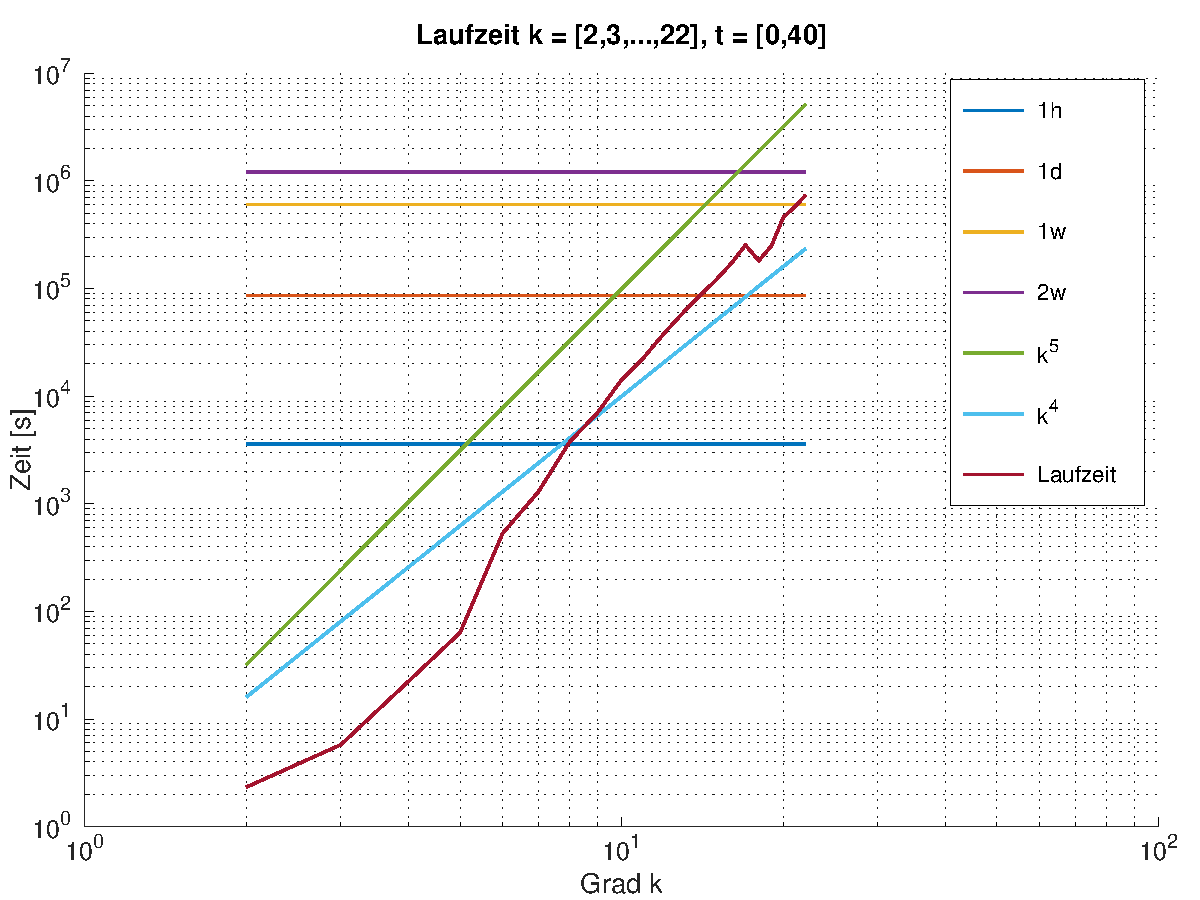
\includegraphics[width=0.49\linewidth]{lorenz2/03-images/timing_40}
	\caption{Laufzeit f"ur Berechnung von eines Lorenzsystems mit Grad $k$}
	\label{figure:lorenz2:timings}
\end{figure}

\begin{figure}
	\centering
	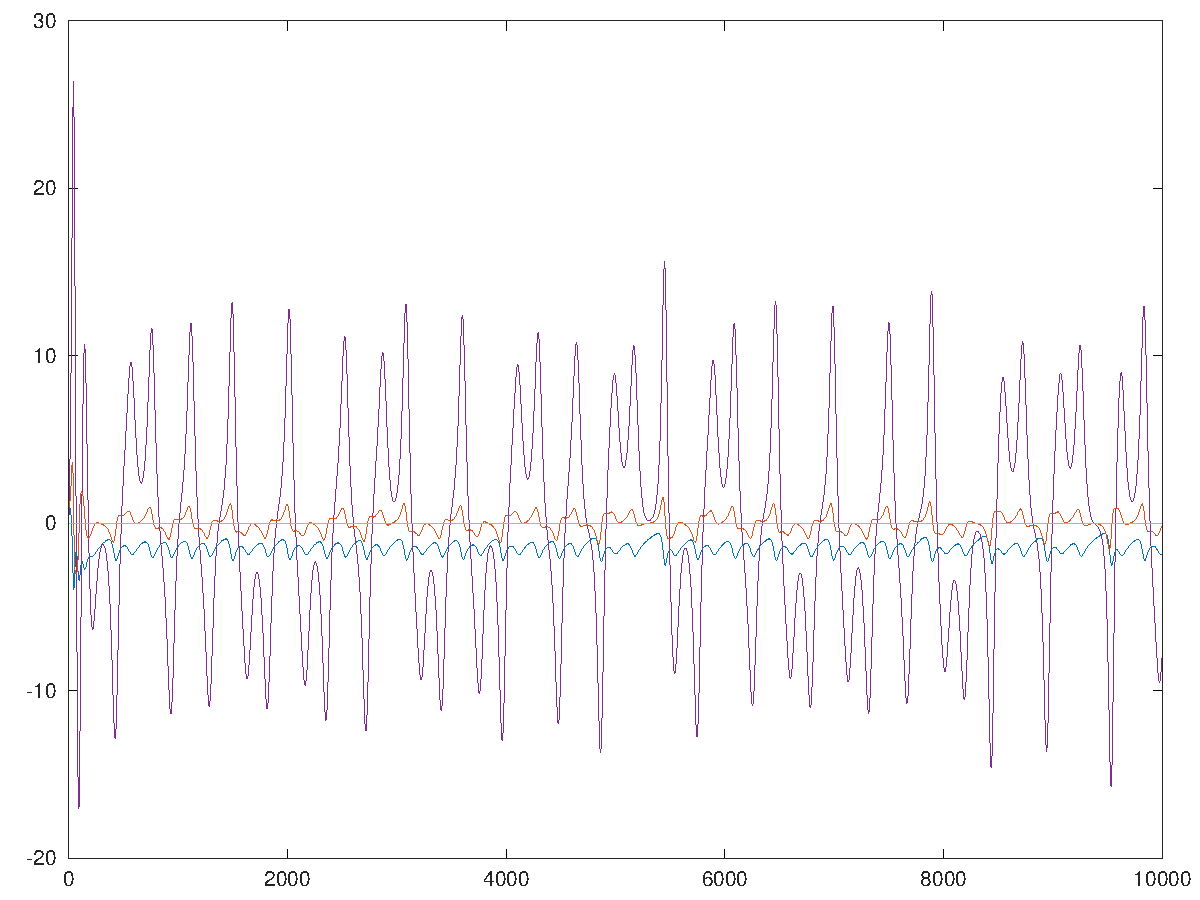
\includegraphics[width=0.49\linewidth]{{lorenz2/03-images/ord2.X}.pdf}
	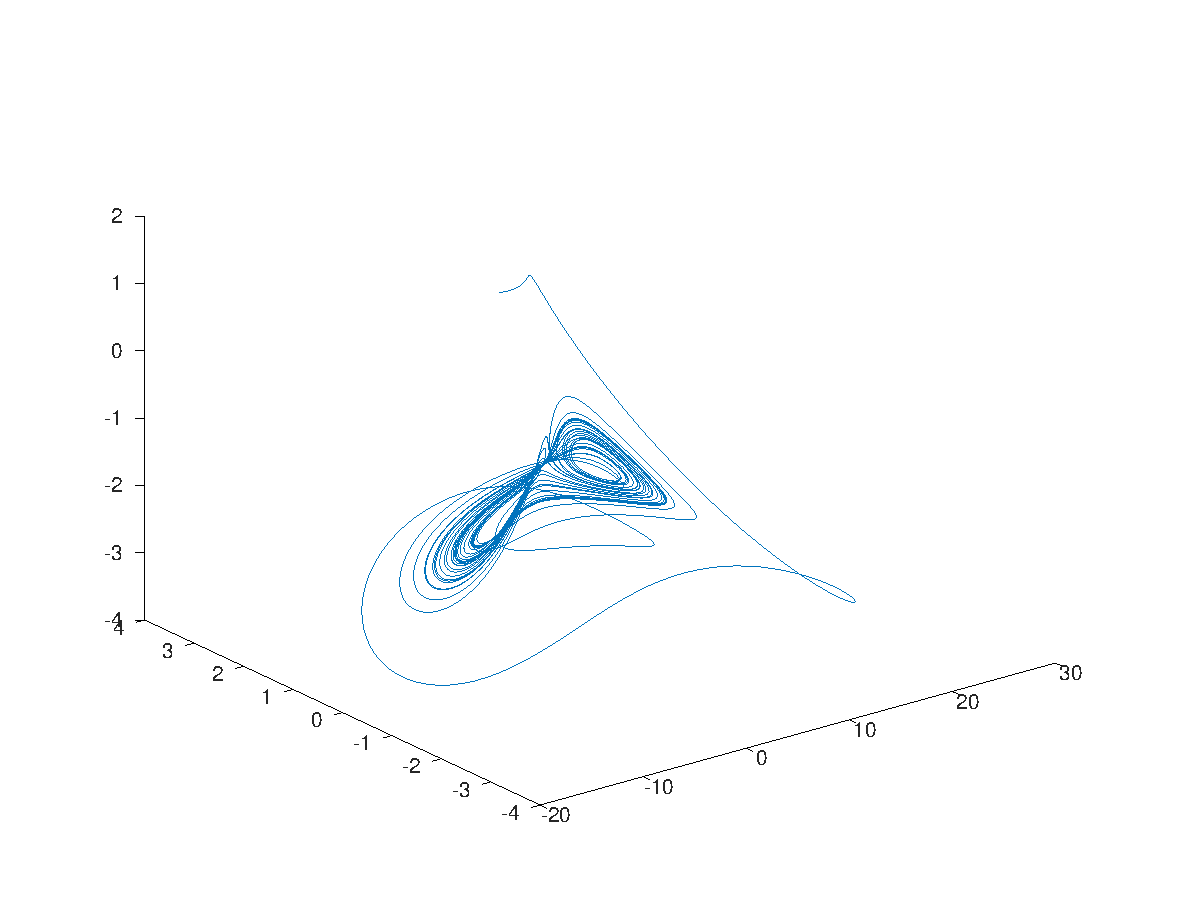
\includegraphics[width=0.49\linewidth]{{lorenz2/03-images/ord2.butterfly}.pdf}
	\caption{Lorenzssystem mit Grad 2}
	\label{figure:lorenz2:systemdeg2}
\end{figure}

\begin{figure}
	\centering
	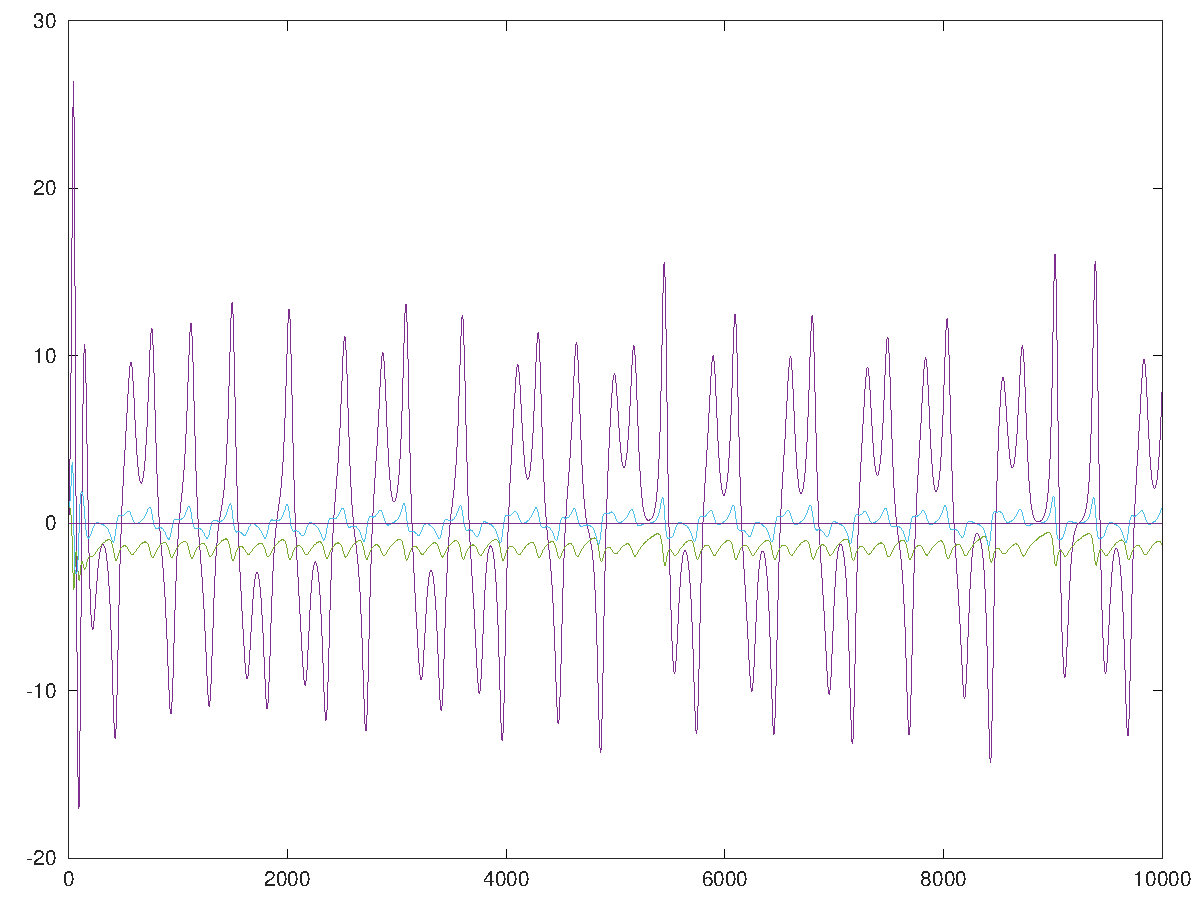
\includegraphics[width=0.49\linewidth]{{lorenz2/03-images/ord3.X}.pdf}
	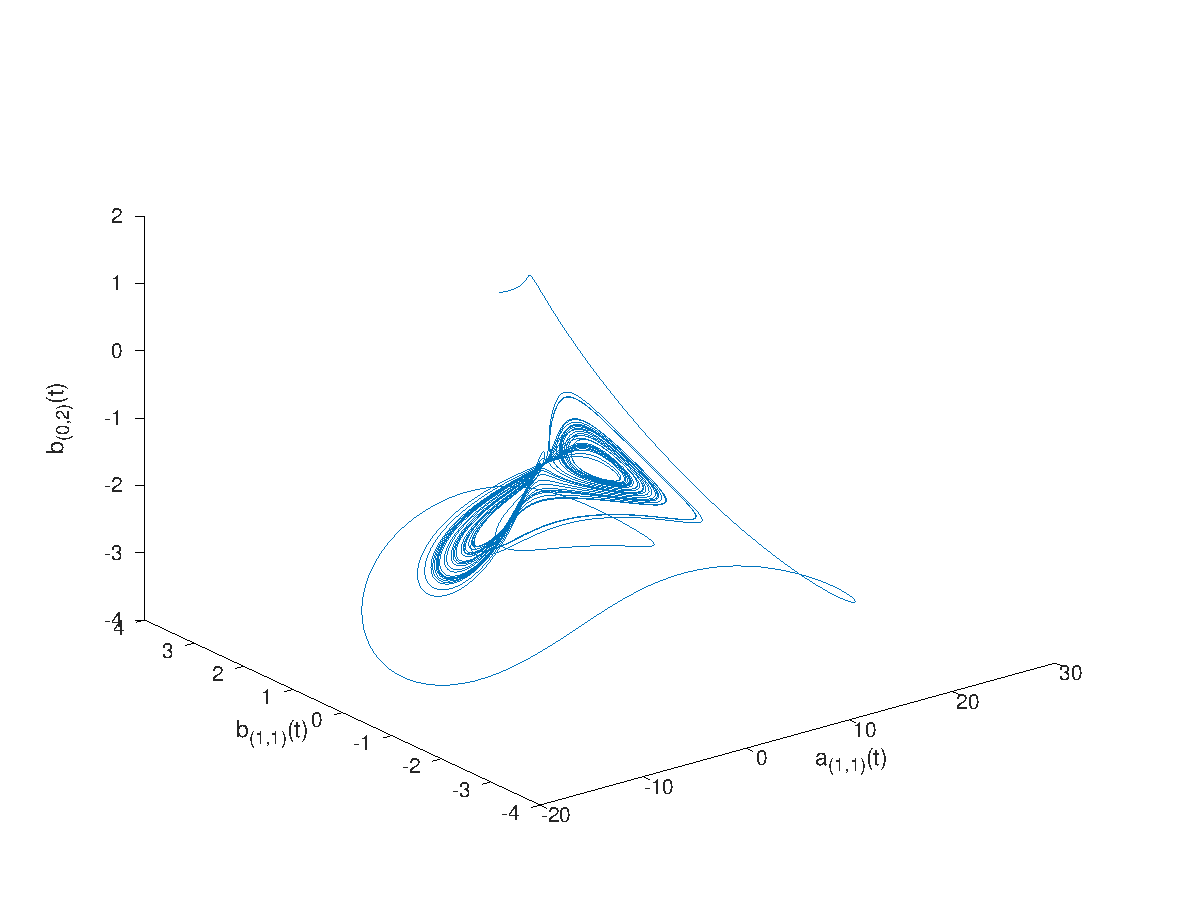
\includegraphics[width=0.49\linewidth]{{lorenz2/03-images/ord3.butterfly}.pdf}
	\caption{Lorenzssystem mit Grad 3}
	\label{figure:lorenz2:systemdeg3}
\end{figure}

\begin{figure}
	\centering
	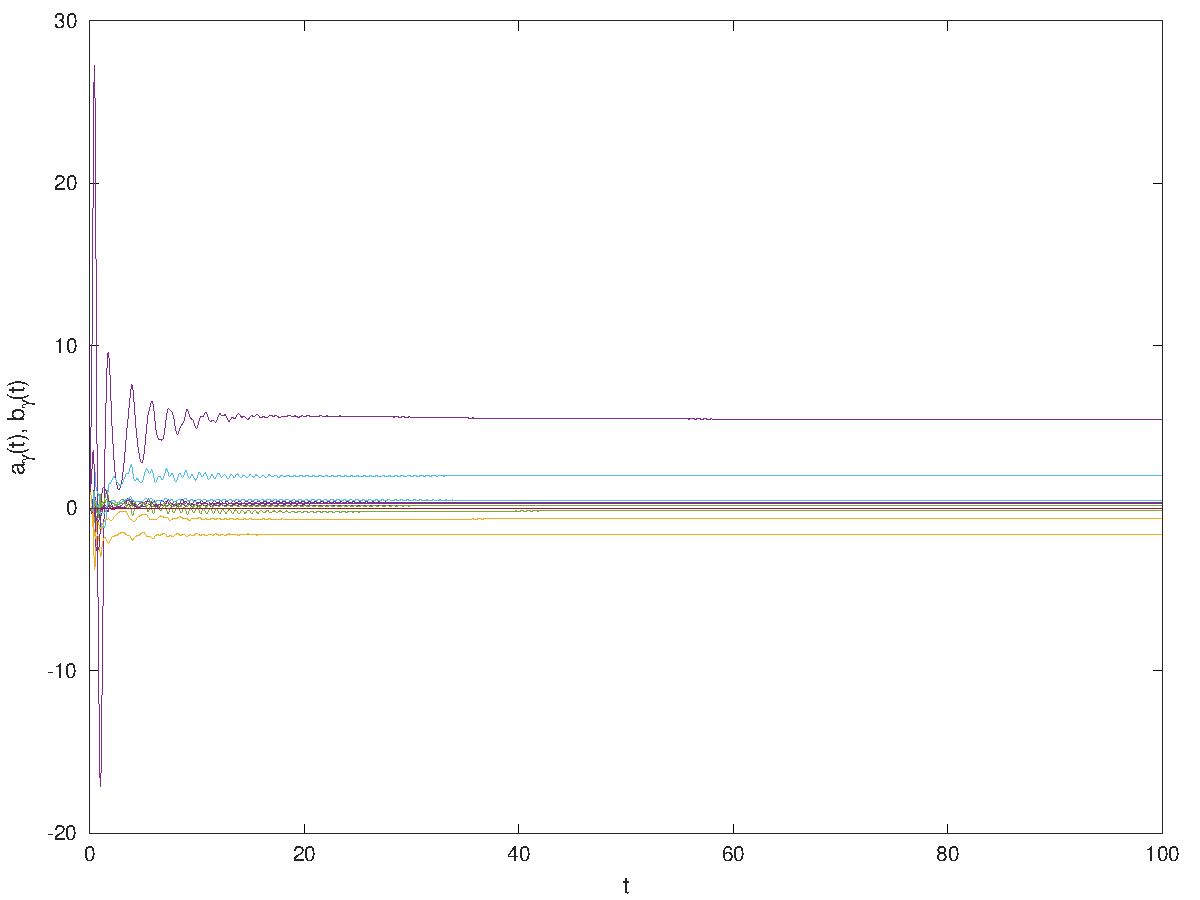
\includegraphics[width=0.49\linewidth]{{lorenz2/03-images/ord4.X}.pdf}
	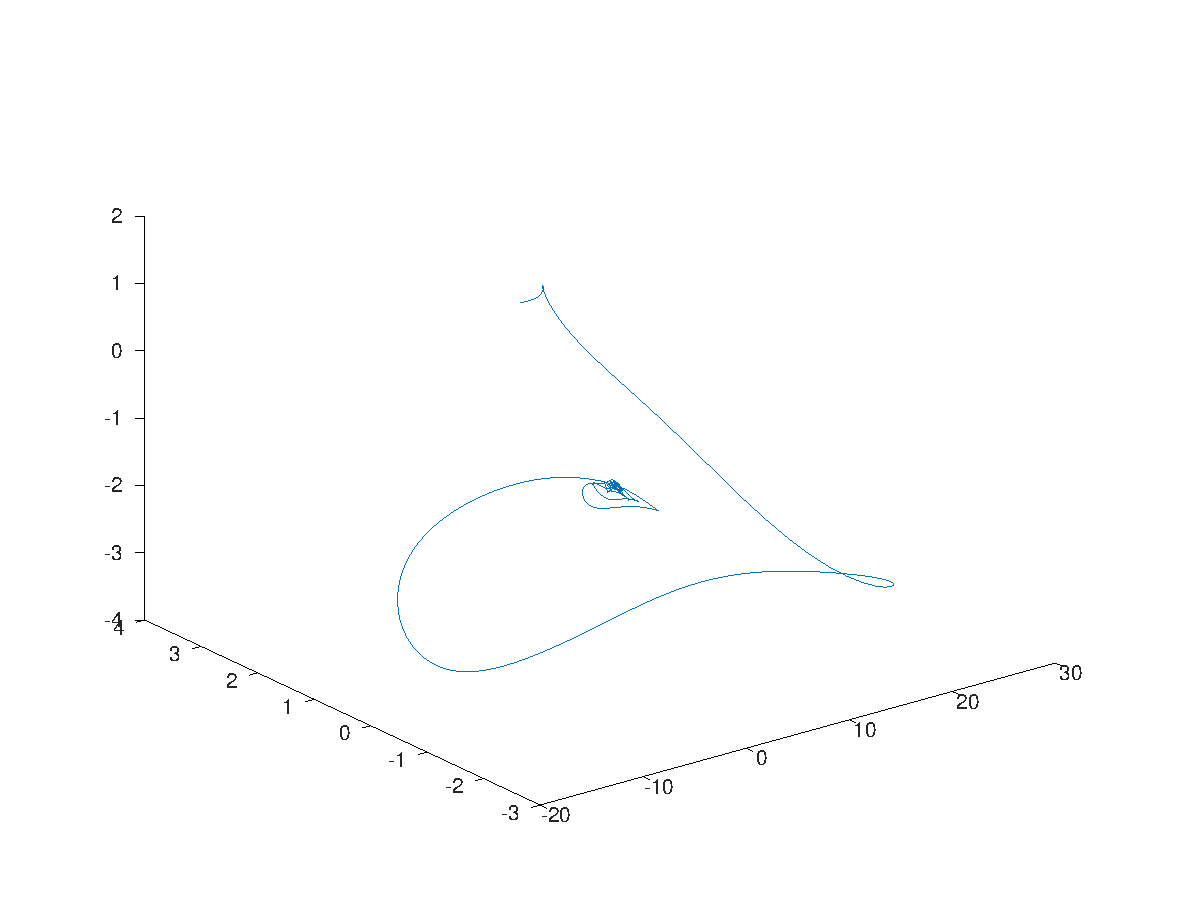
\includegraphics[width=0.49\linewidth]{{lorenz2/03-images/ord4.butterfly}.pdf}
	\caption{Lorenzssystem mit Grad 4}
	\label{figure:lorenz2:systemdeg4}
\end{figure}

\begin{figure}
	\centering
	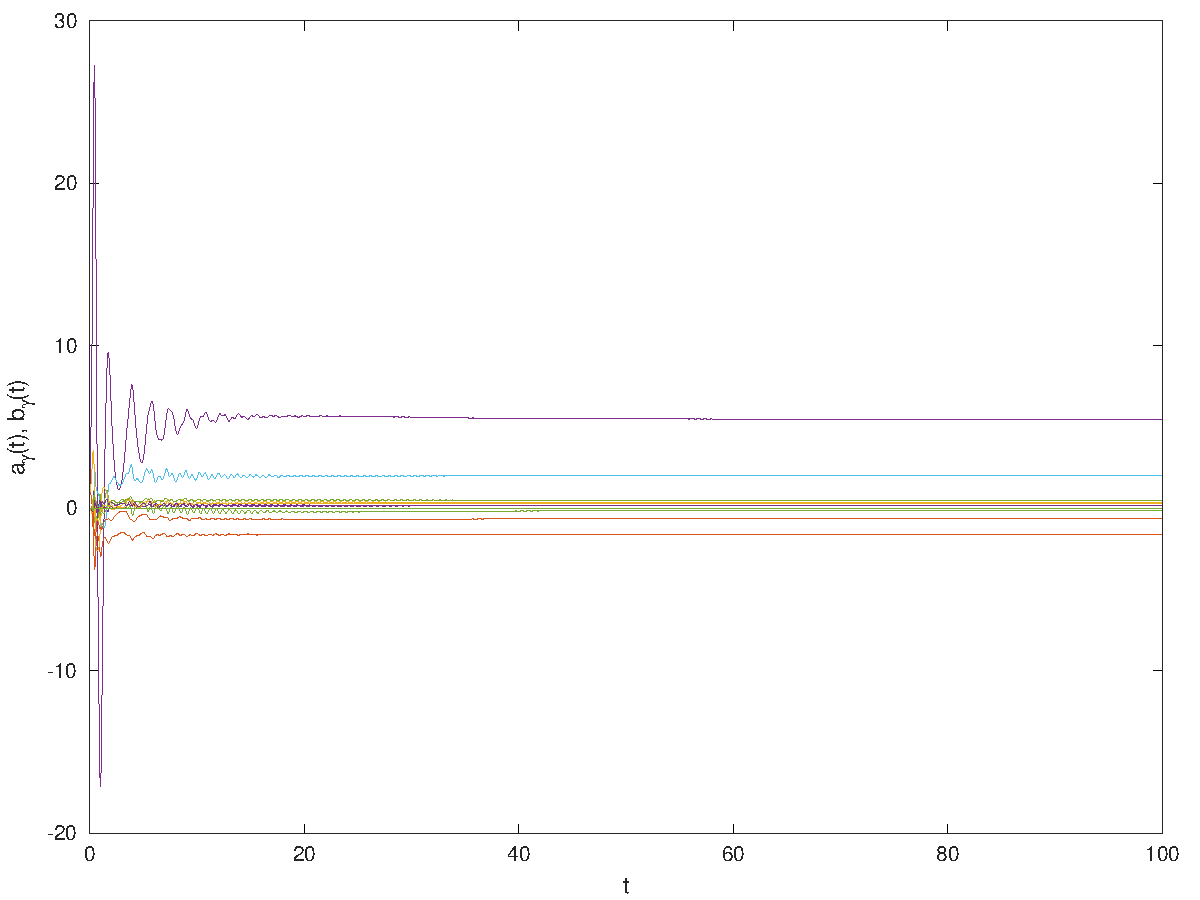
\includegraphics[width=0.49\linewidth]{{lorenz2/03-images/ord5.X}.pdf}
	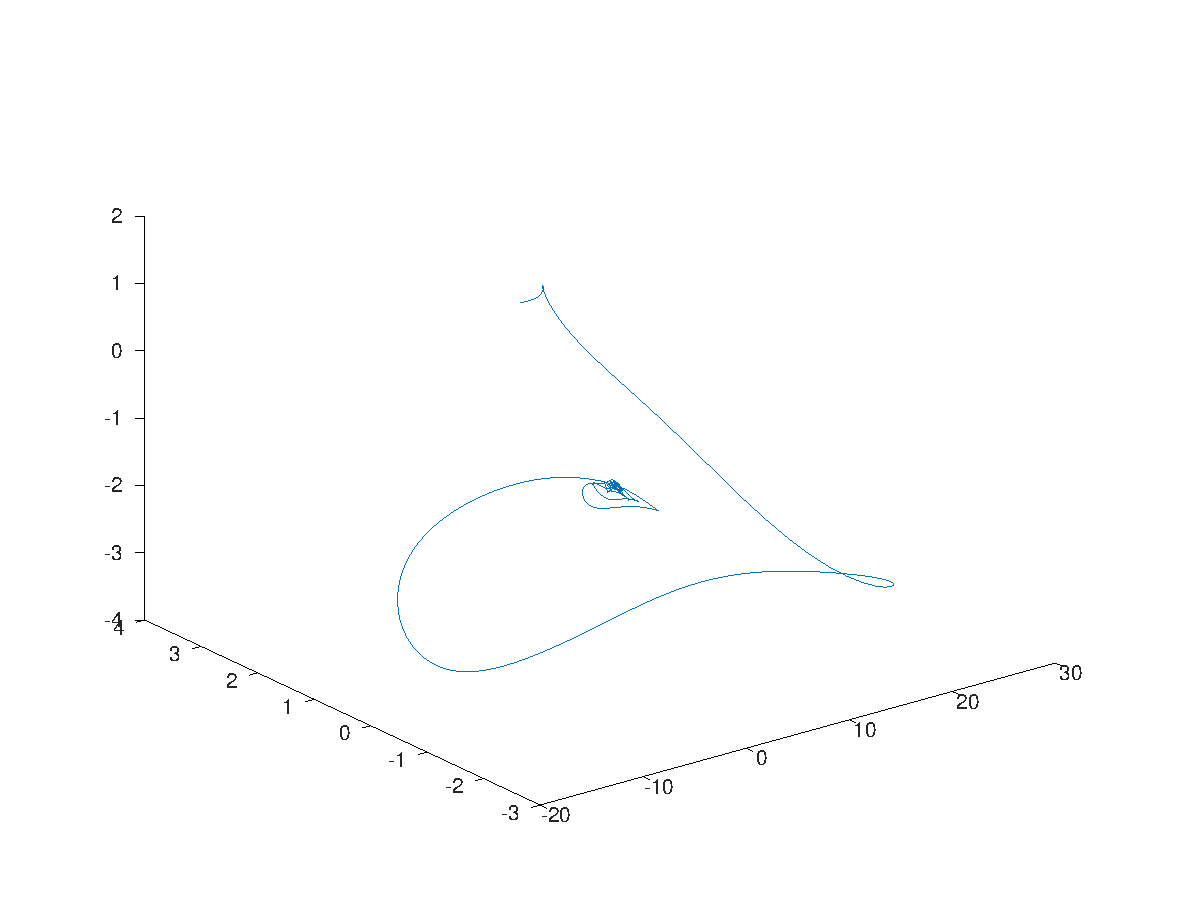
\includegraphics[width=0.49\linewidth]{{lorenz2/03-images/ord5.butterfly}.pdf}
	\caption{Lorenzssystem mit Grad 5}
	\label{figure:lorenz2:systemdeg5}
\end{figure}

\begin{figure}
	\centering
	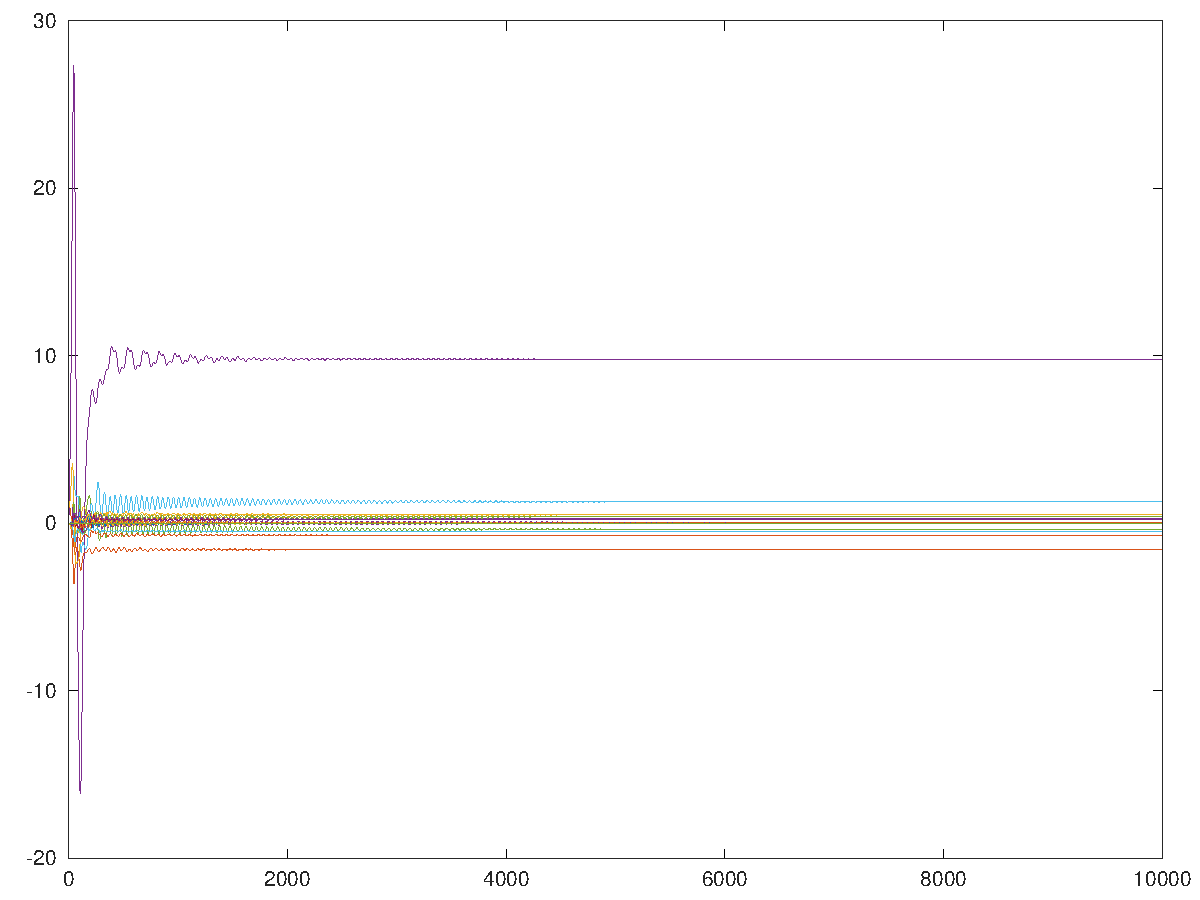
\includegraphics[width=0.49\linewidth]{{lorenz2/03-images/ord6.X}.pdf}
	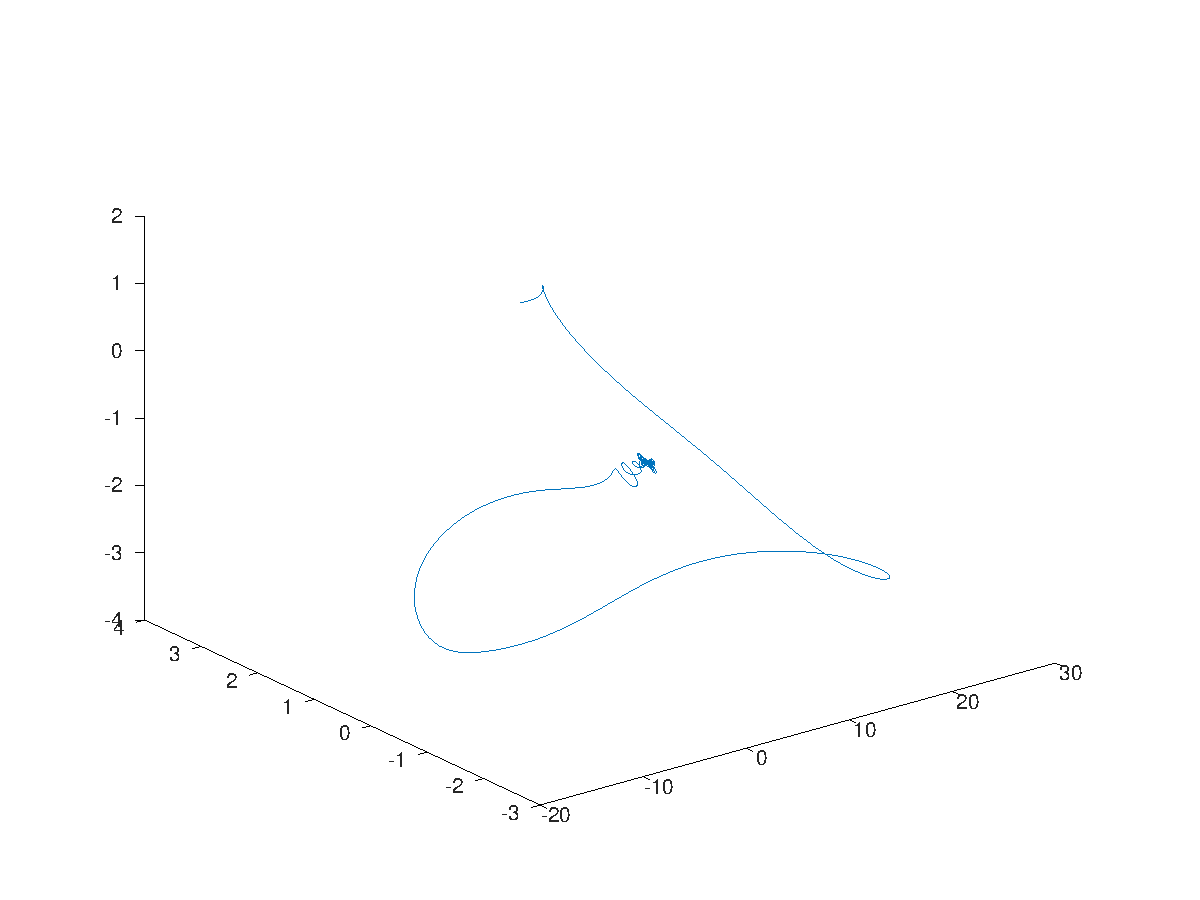
\includegraphics[width=0.49\linewidth]{{lorenz2/03-images/ord6.butterfly}.pdf}
	\caption{Lorenzssystem mit Grad 6}
	\label{figure:lorenz2:systemdeg6}
\end{figure}

\begin{figure}
	\centering
	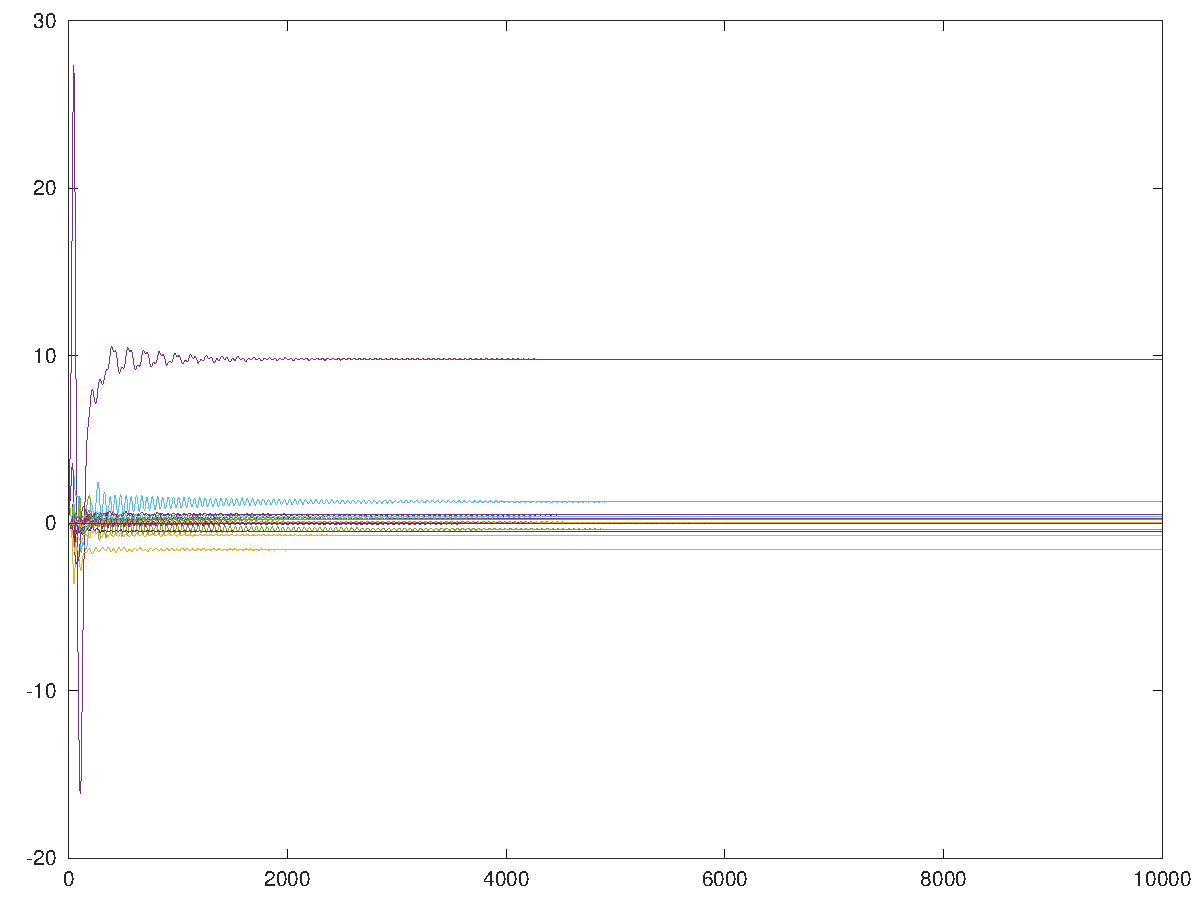
\includegraphics[width=0.49\linewidth]{{lorenz2/03-images/ord7.X}.pdf}
	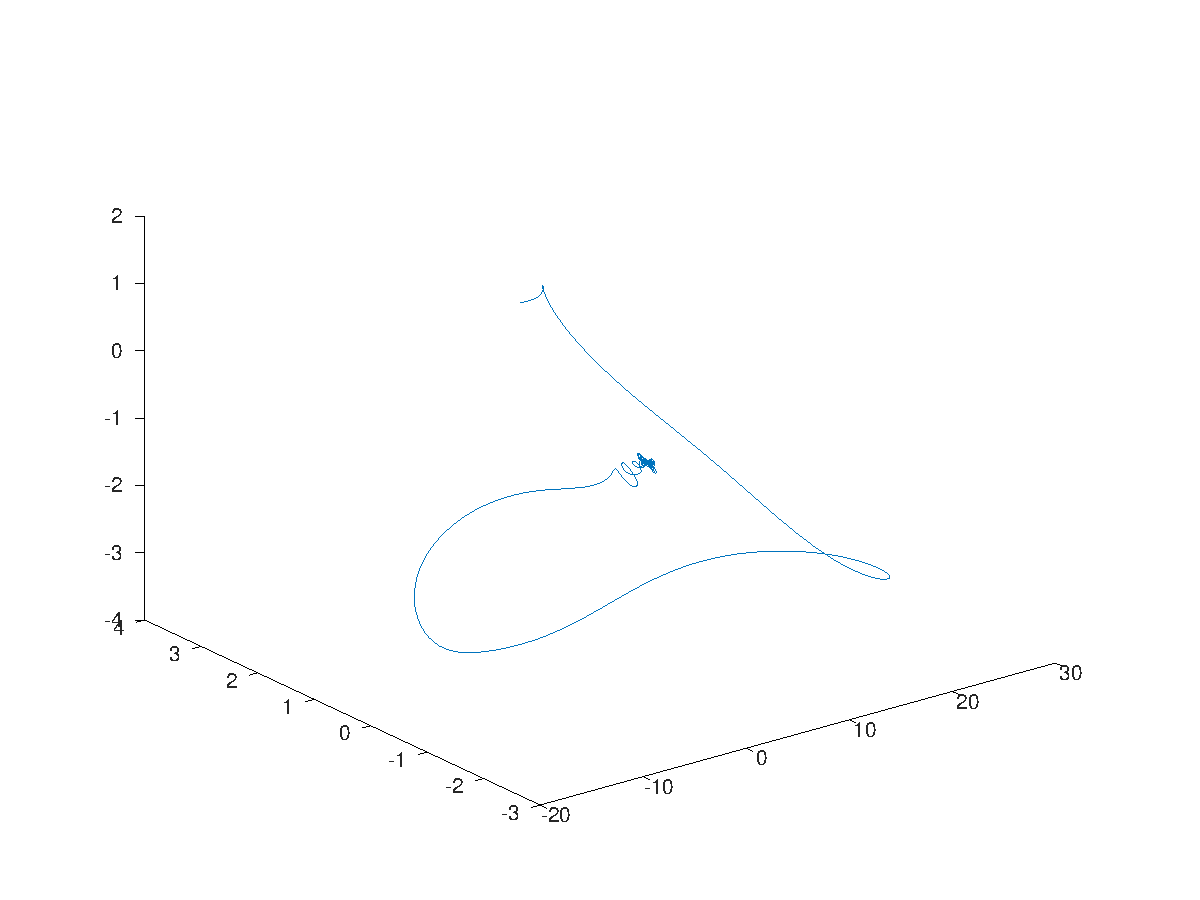
\includegraphics[width=0.49\linewidth]{{lorenz2/03-images/ord7.butterfly}.pdf}
	\caption{Lorenzssystem mit Grad 7}
	\label{figure:lorenz2:systemdeg7}
\end{figure}

\begin{figure}
	\centering
	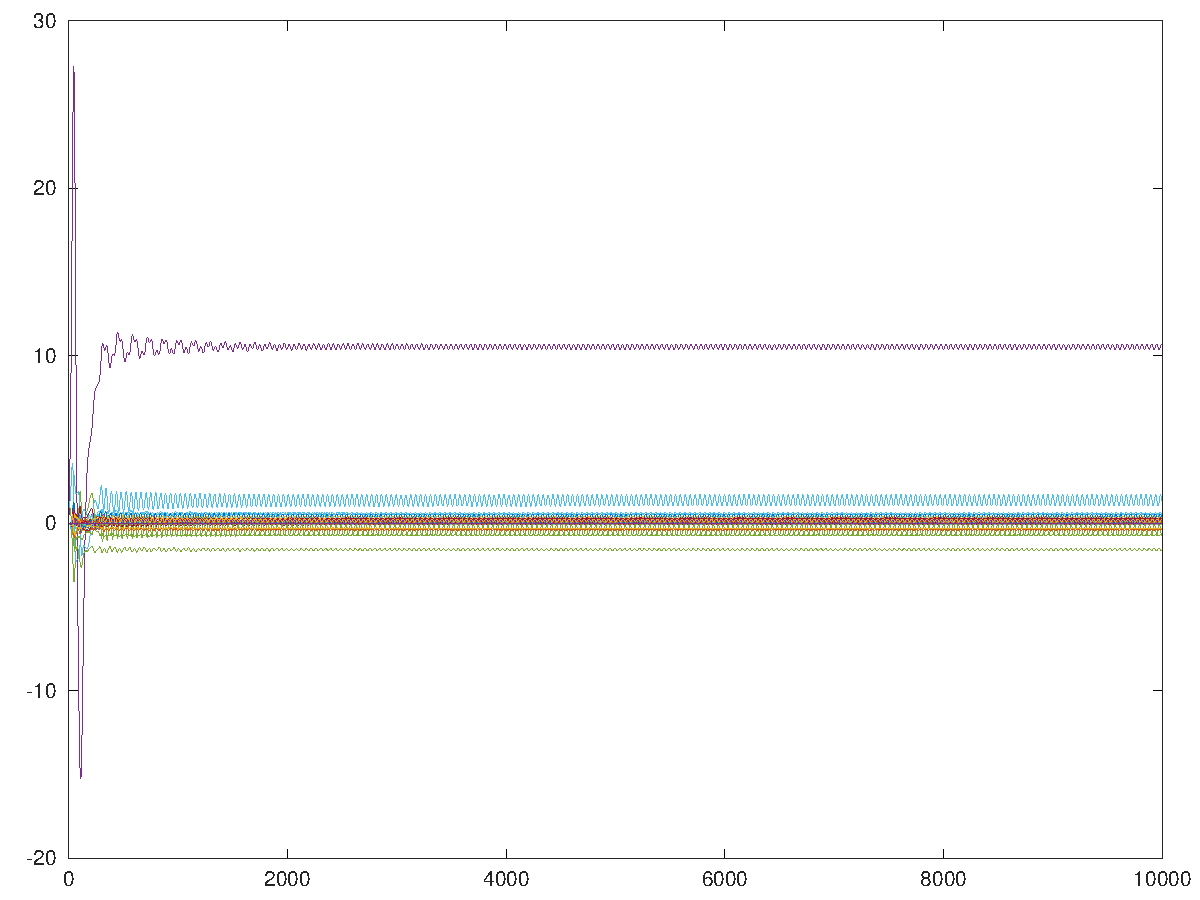
\includegraphics[width=0.49\linewidth]{{lorenz2/03-images/ord8.X}.pdf}
	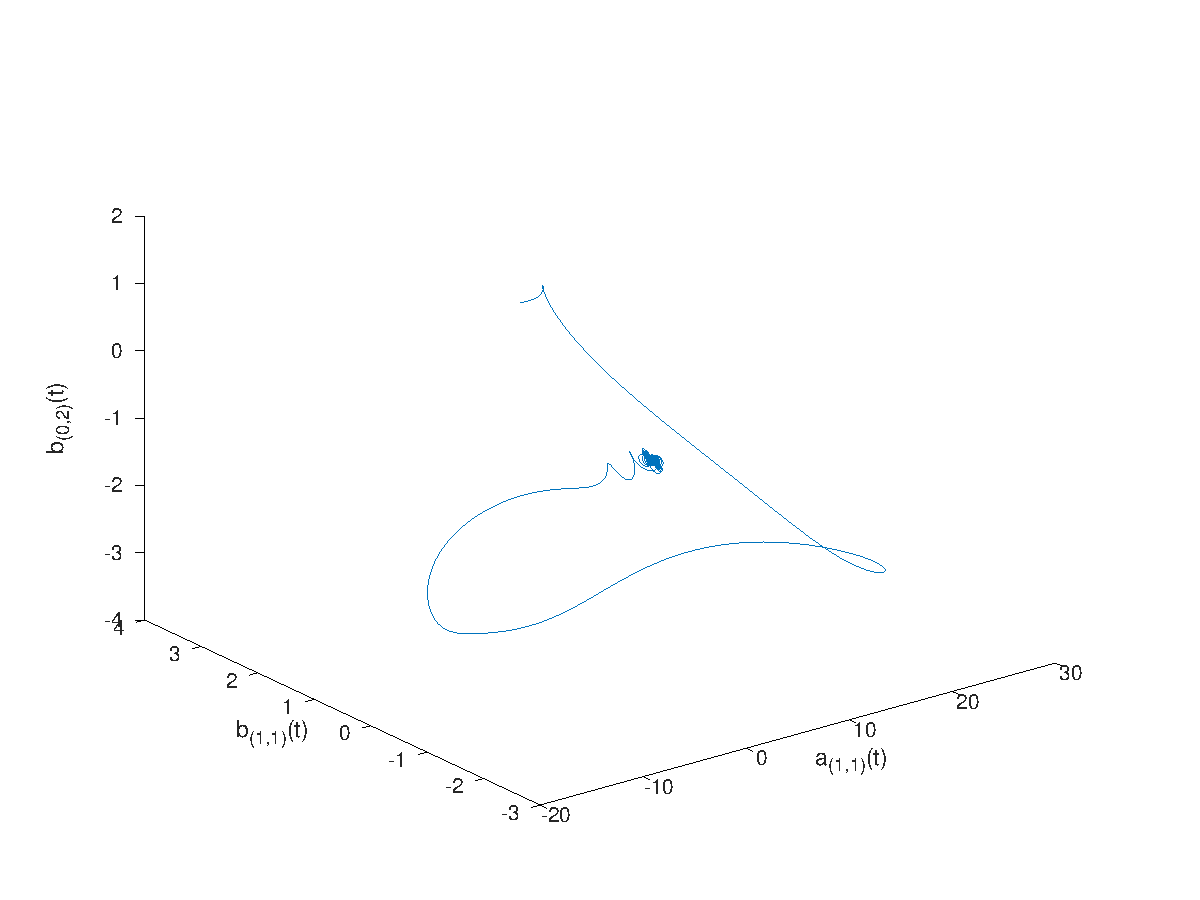
\includegraphics[width=0.49\linewidth]{{lorenz2/03-images/ord8.butterfly}.pdf}
	\caption{Lorenzssystem mit Grad 8}
	\label{figure:lorenz2:systemdeg8}
\end{figure}

\begin{figure}
	\centering
	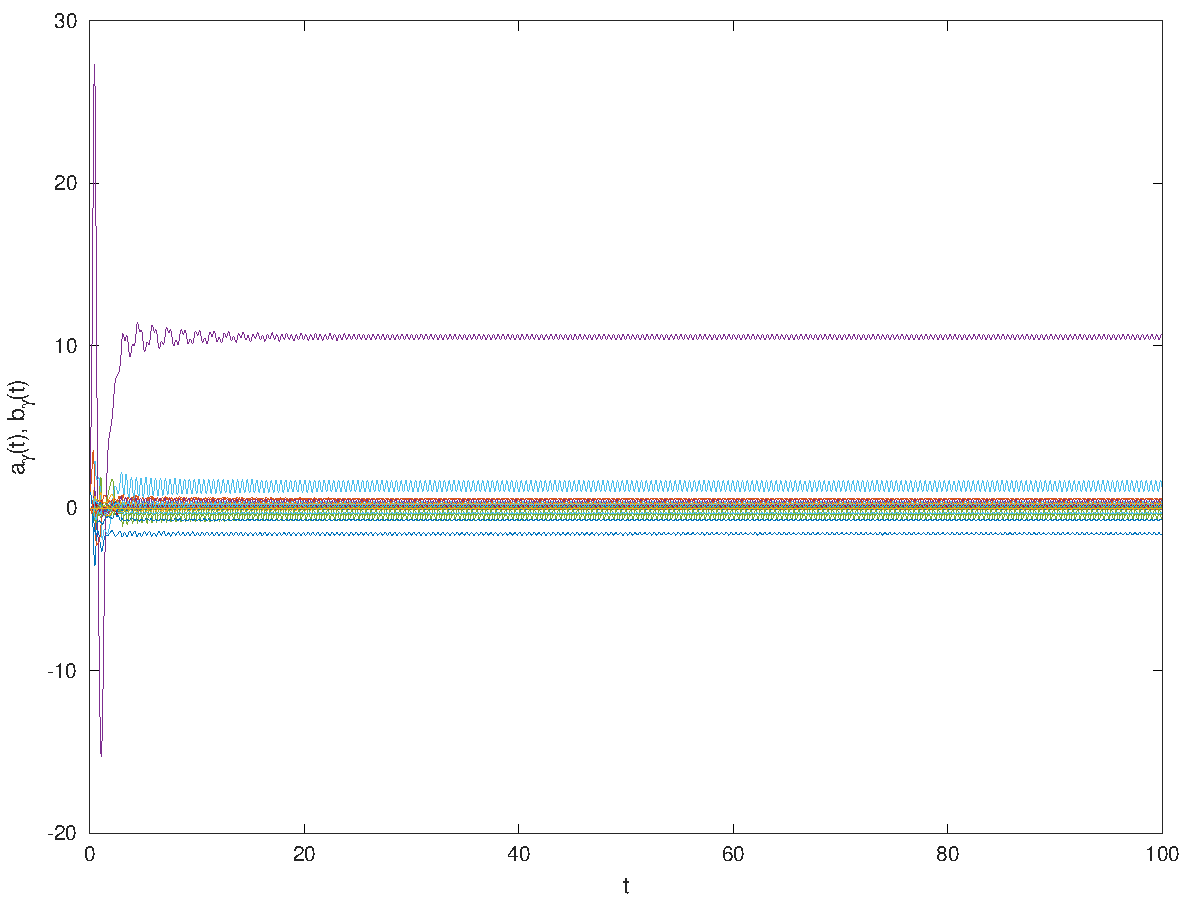
\includegraphics[width=0.49\linewidth]{{lorenz2/03-images/ord9.X}.pdf}
	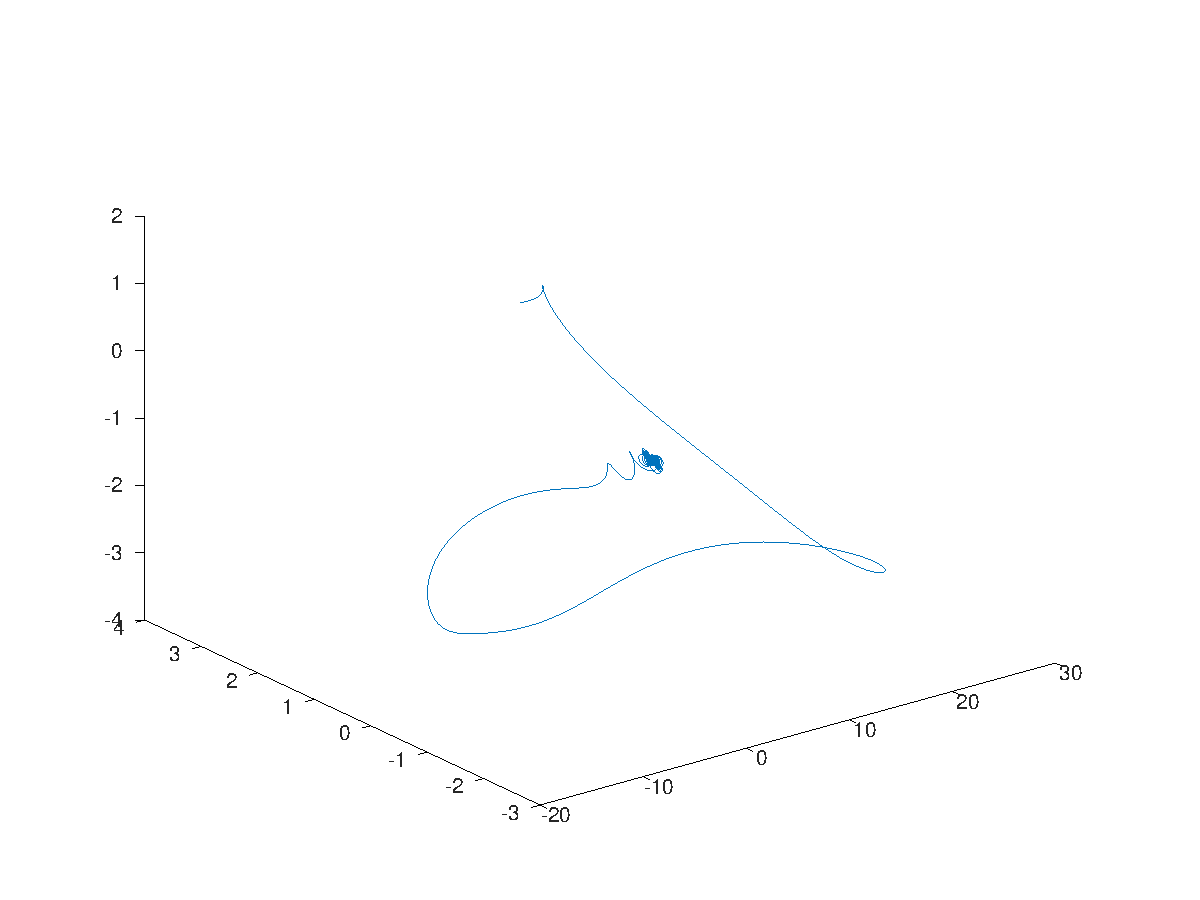
\includegraphics[width=0.49\linewidth]{{lorenz2/03-images/ord9.butterfly}.pdf}
	\caption{Lorenzssystem mit Grad 9}
	\label{figure:lorenz2:systemdeg9}
\end{figure}

\begin{figure}
	\centering
	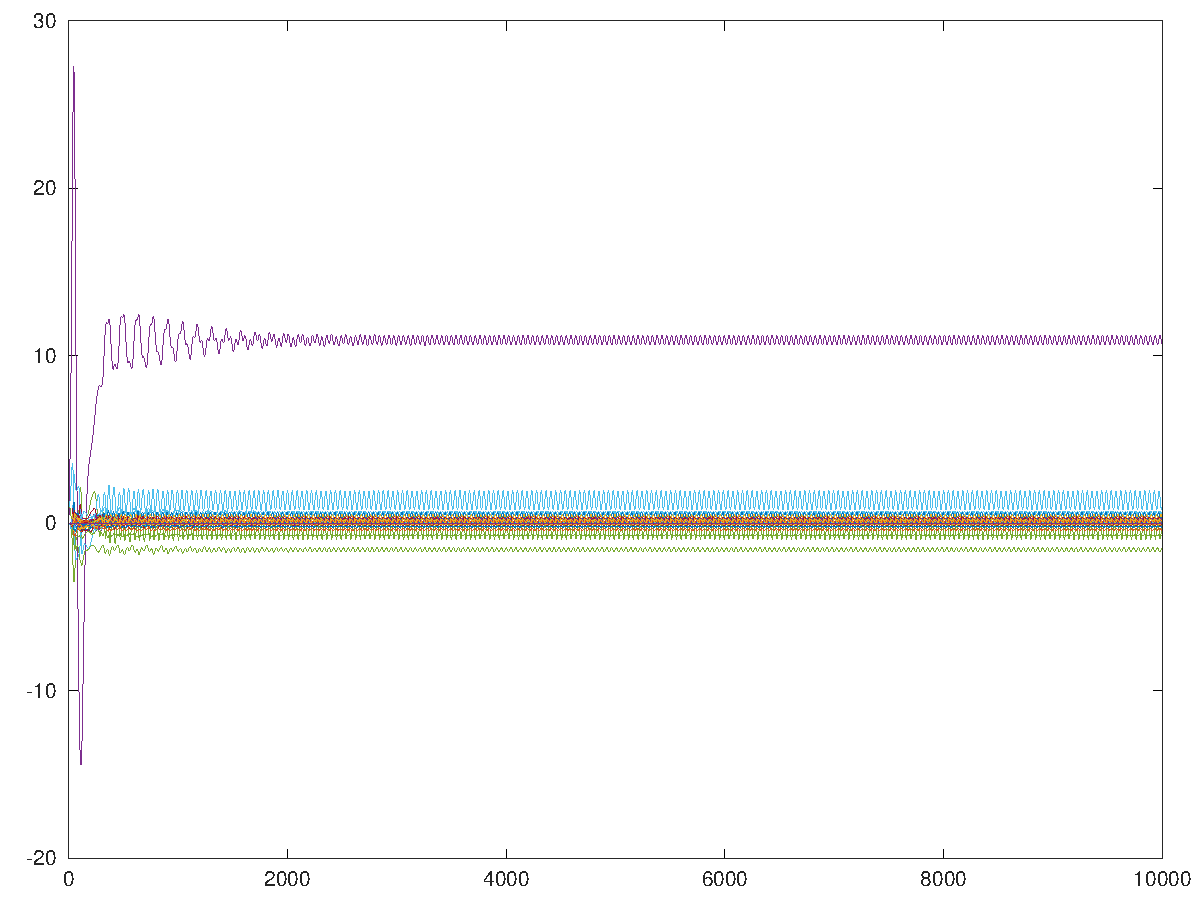
\includegraphics[width=0.49\linewidth]{{lorenz2/03-images/ord10.X}.pdf}
	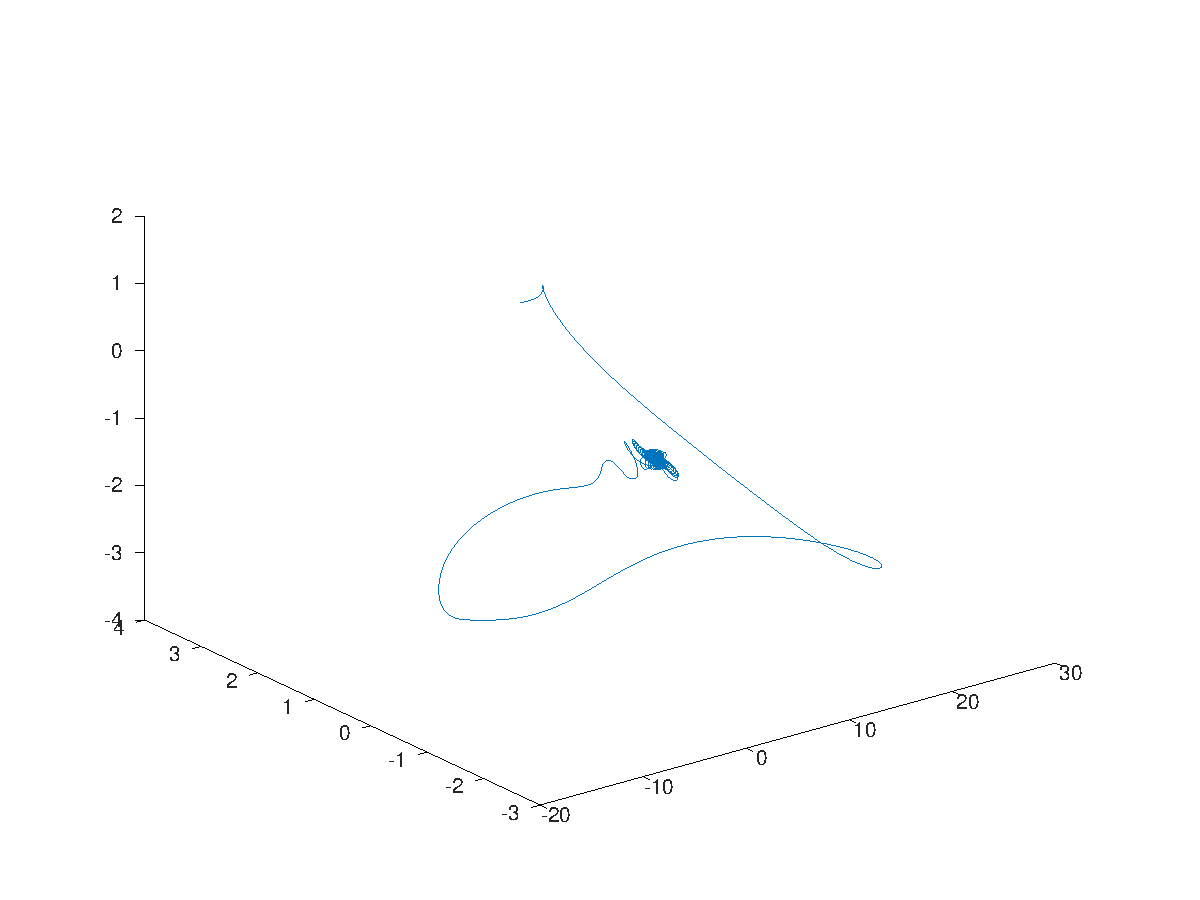
\includegraphics[width=0.49\linewidth]{{lorenz2/03-images/ord10.butterfly}.pdf}
	\caption{Lorenzssystem mit Grad 10, $t = [0,100]$}
	\label{figure:lorenz2:systemdeg10}
\end{figure}

\begin{figure}
	\centering
	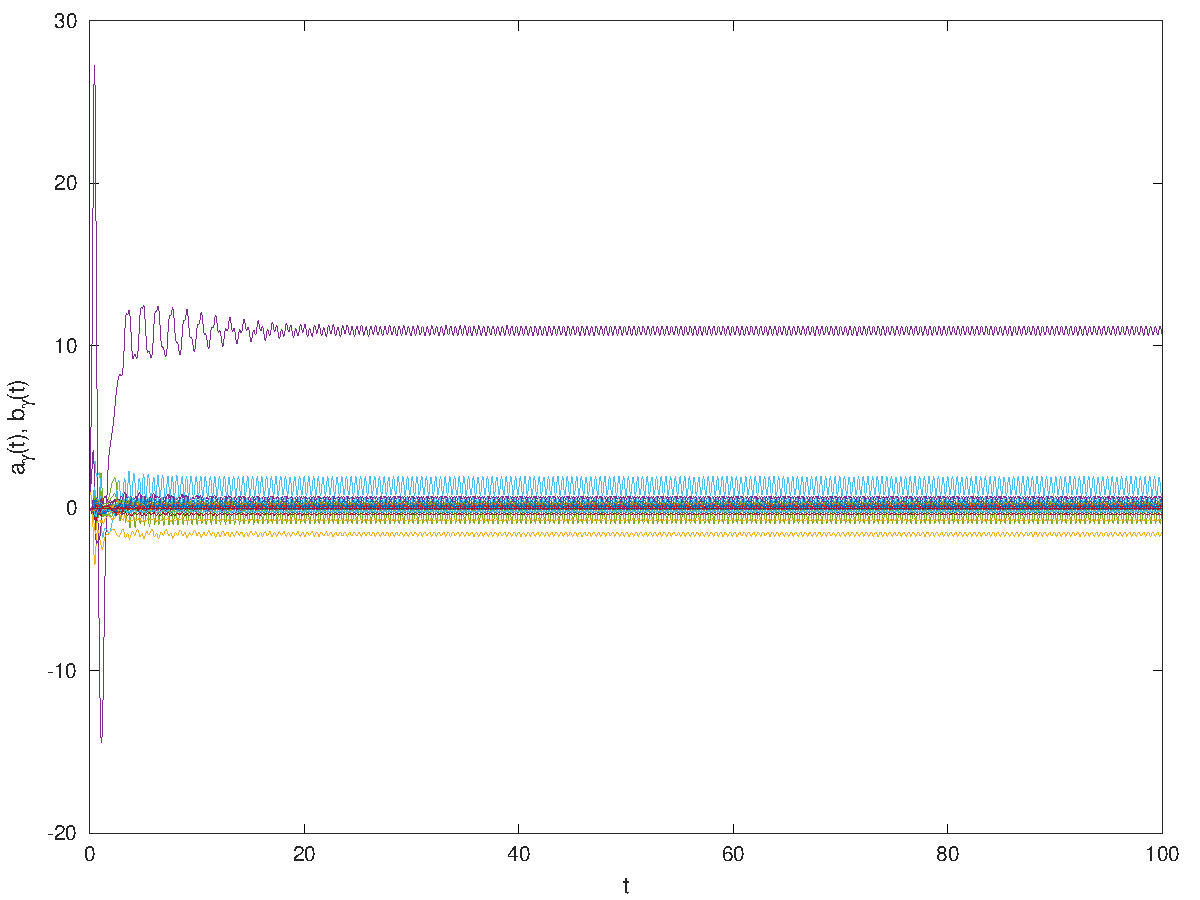
\includegraphics[width=0.49\linewidth]{{lorenz2/03-images/ord11.X}.pdf}
	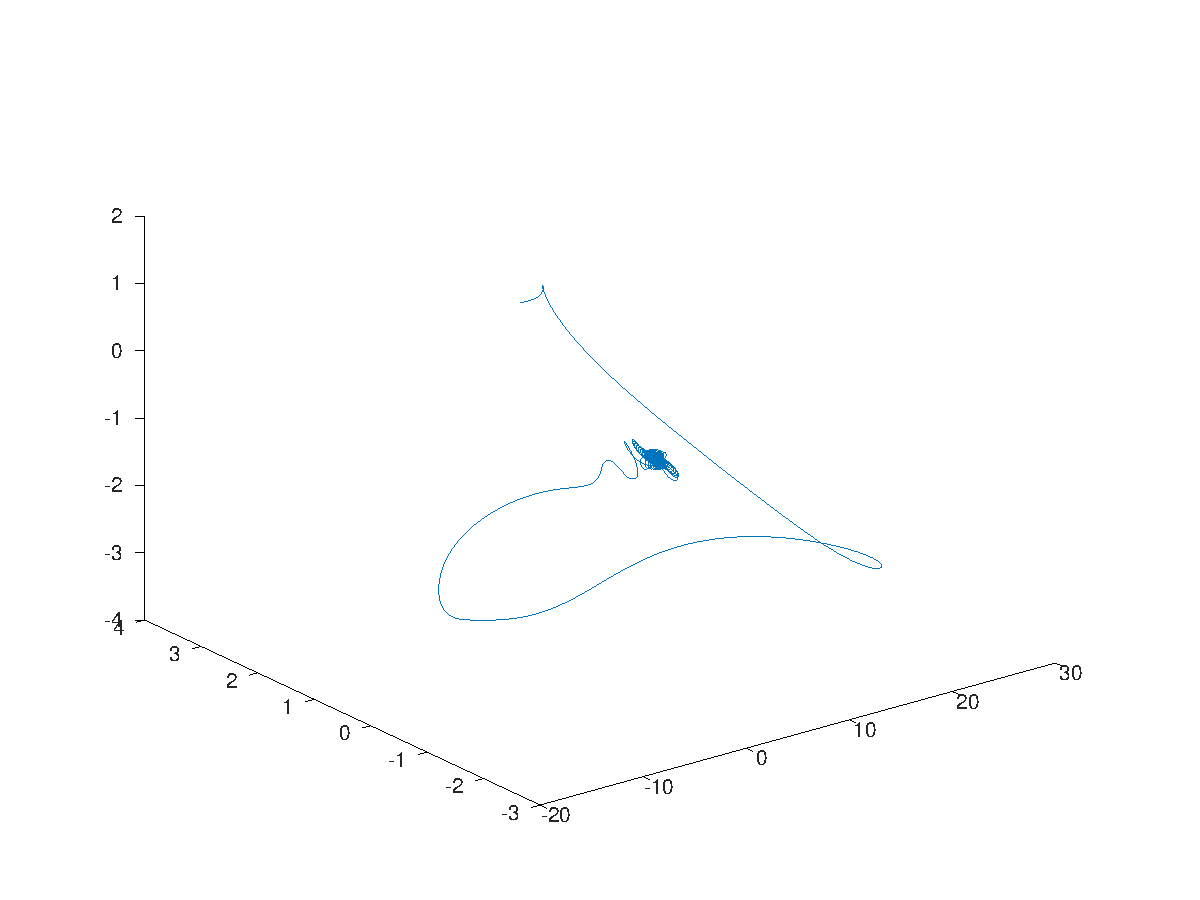
\includegraphics[width=0.49\linewidth]{{lorenz2/03-images/ord11.butterfly}.pdf}
	\caption{Lorenzssystem mit Grad 11, $t = [0,100]$}
	\label{figure:lorenz2:systemdeg11}
\end{figure}

\begin{figure}
	\centering
	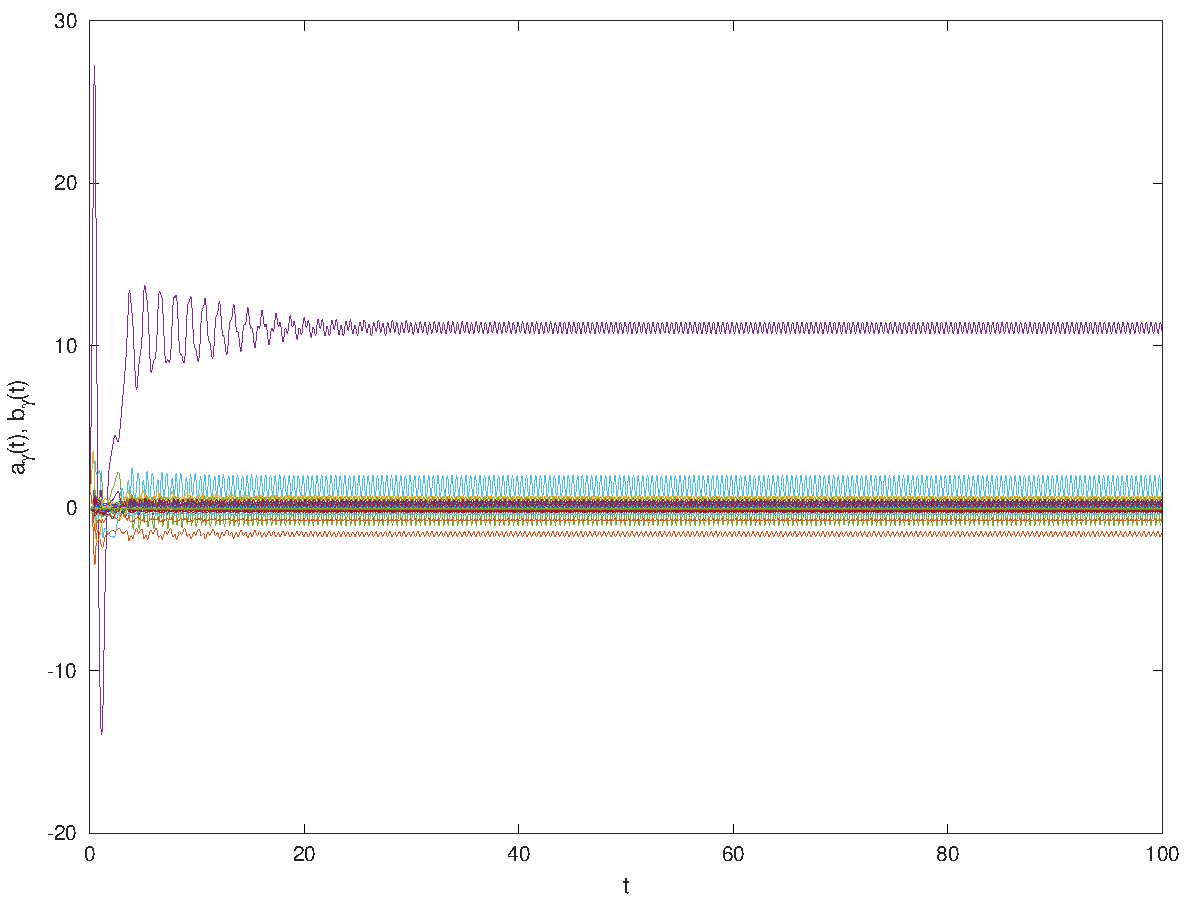
\includegraphics[width=0.49\linewidth]{{lorenz2/03-images/ord12.X}.pdf}
	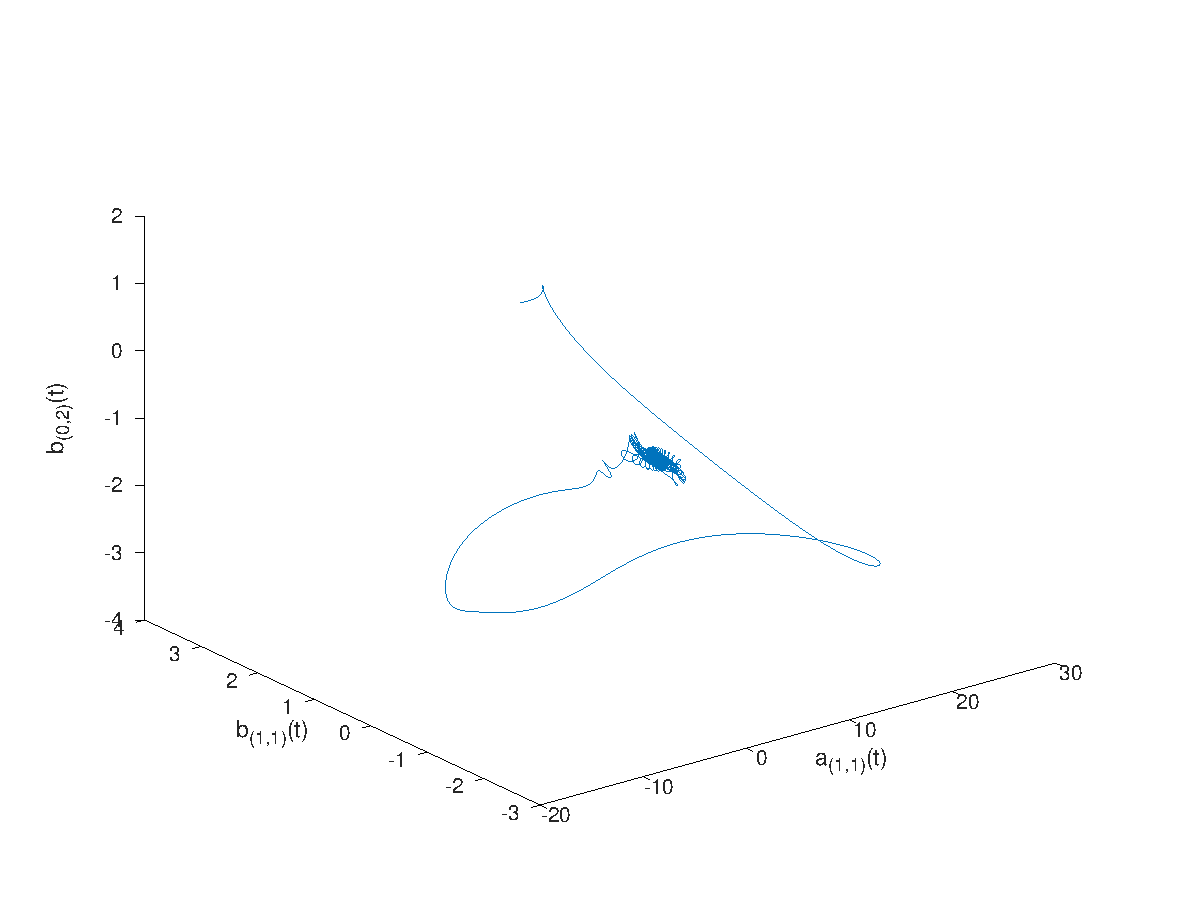
\includegraphics[width=0.49\linewidth]{{lorenz2/03-images/ord12.butterfly}.pdf}
	\caption{Lorenzssystem mit Grad 12, $t = [0,100]$}
	\label{figure:lorenz2:systemdeg12}
\end{figure}

\begin{figure}
	\centering
	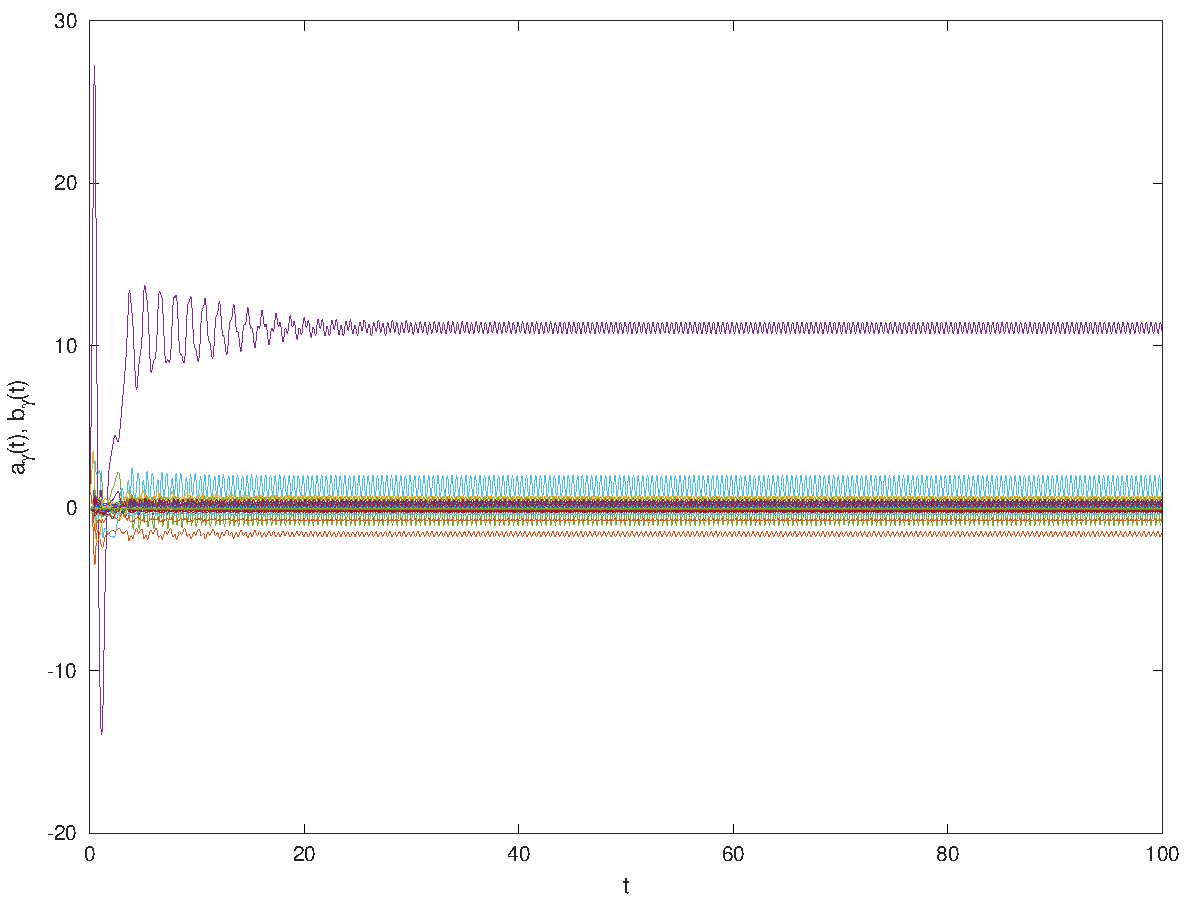
\includegraphics[width=0.49\linewidth]{{lorenz2/03-images/ord13.X}.pdf}
	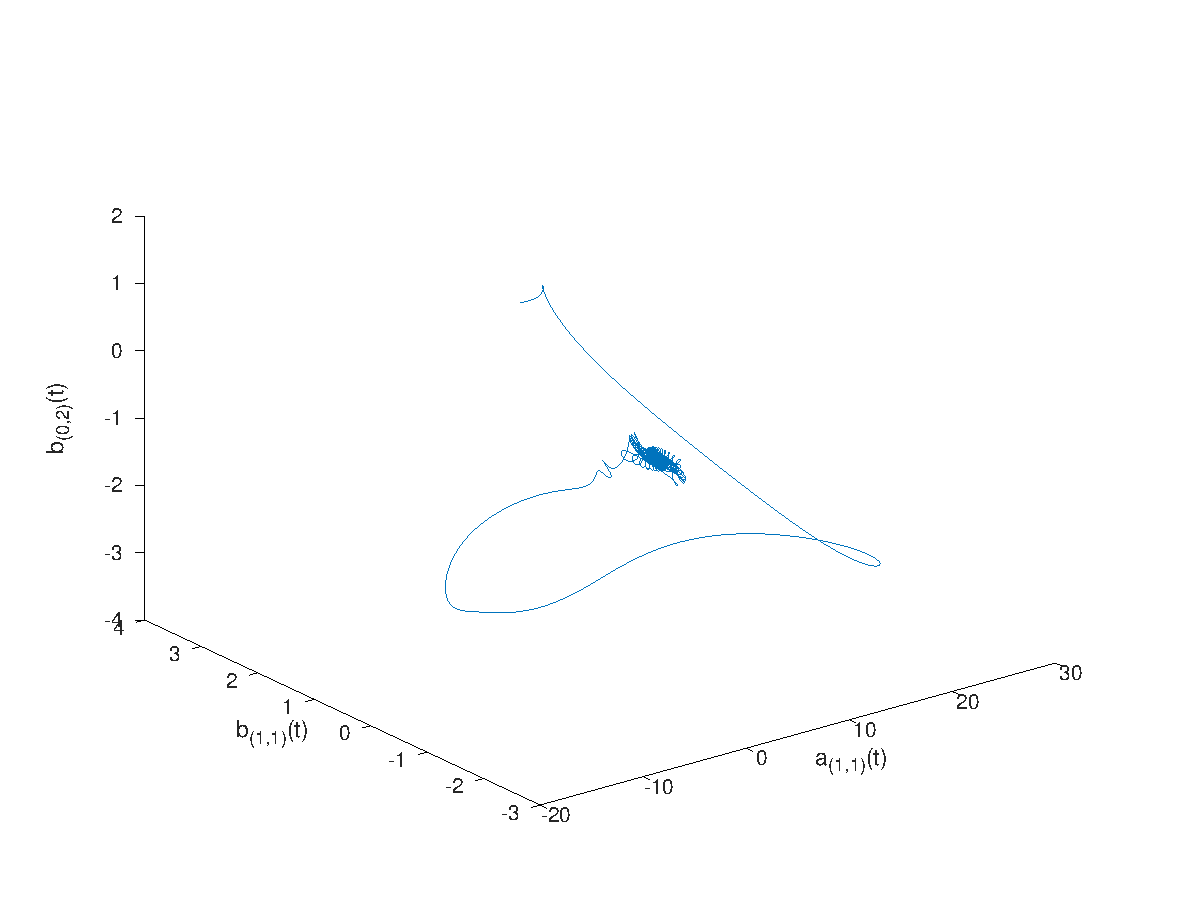
\includegraphics[width=0.49\linewidth]{{lorenz2/03-images/ord13.butterfly}.pdf}
	\caption{Lorenzssystem mit Grad 13, $t = [0,100]$}
	\label{figure:lorenz2:systemdeg13}
\end{figure}

\begin{figure}
	\centering
	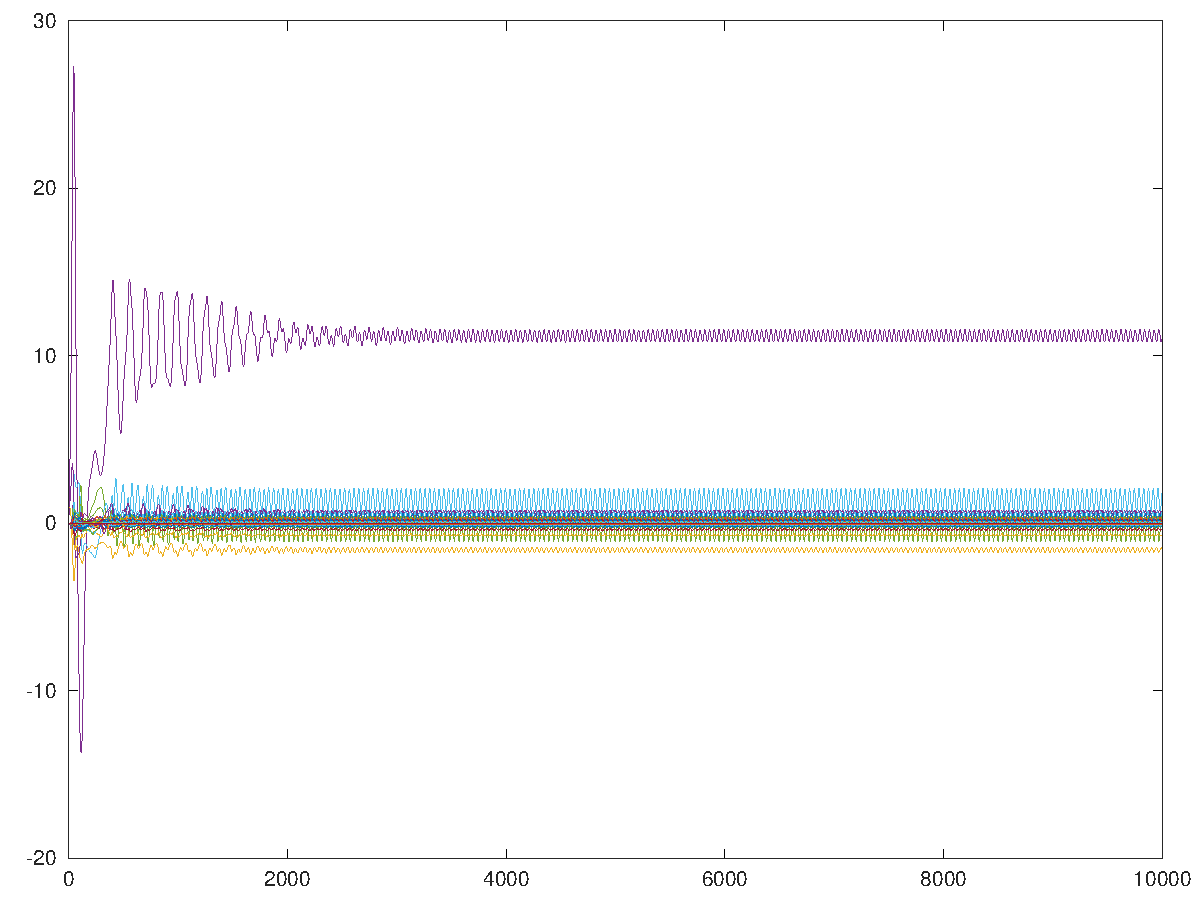
\includegraphics[width=0.49\linewidth]{{lorenz2/03-images/ord14.X}.pdf}
	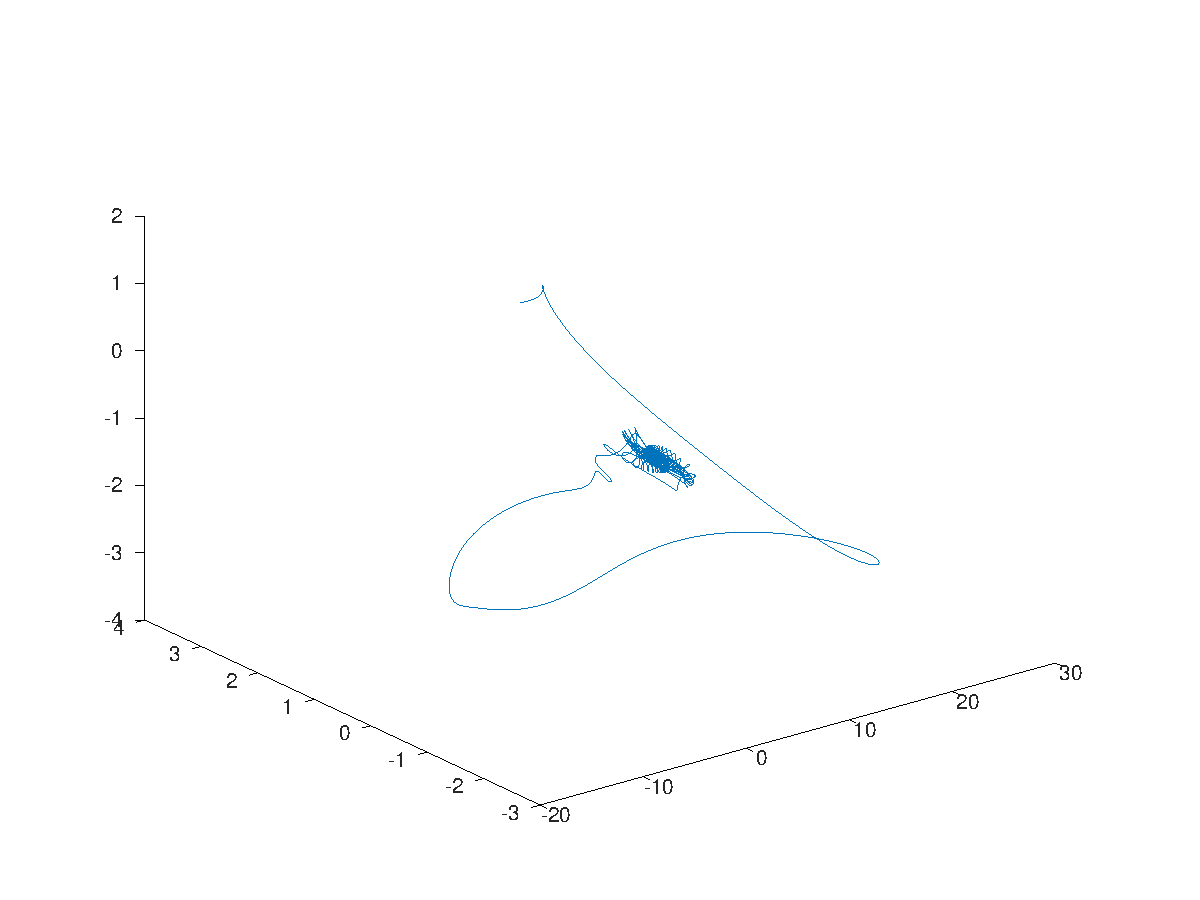
\includegraphics[width=0.49\linewidth]{{lorenz2/03-images/ord14.butterfly}.pdf}
	\caption{Lorenzssystem mit Grad 14, $t = [0,100]$}
	\label{figure:lorenz2:systemdeg14}
\end{figure}

\begin{figure}
	\centering
	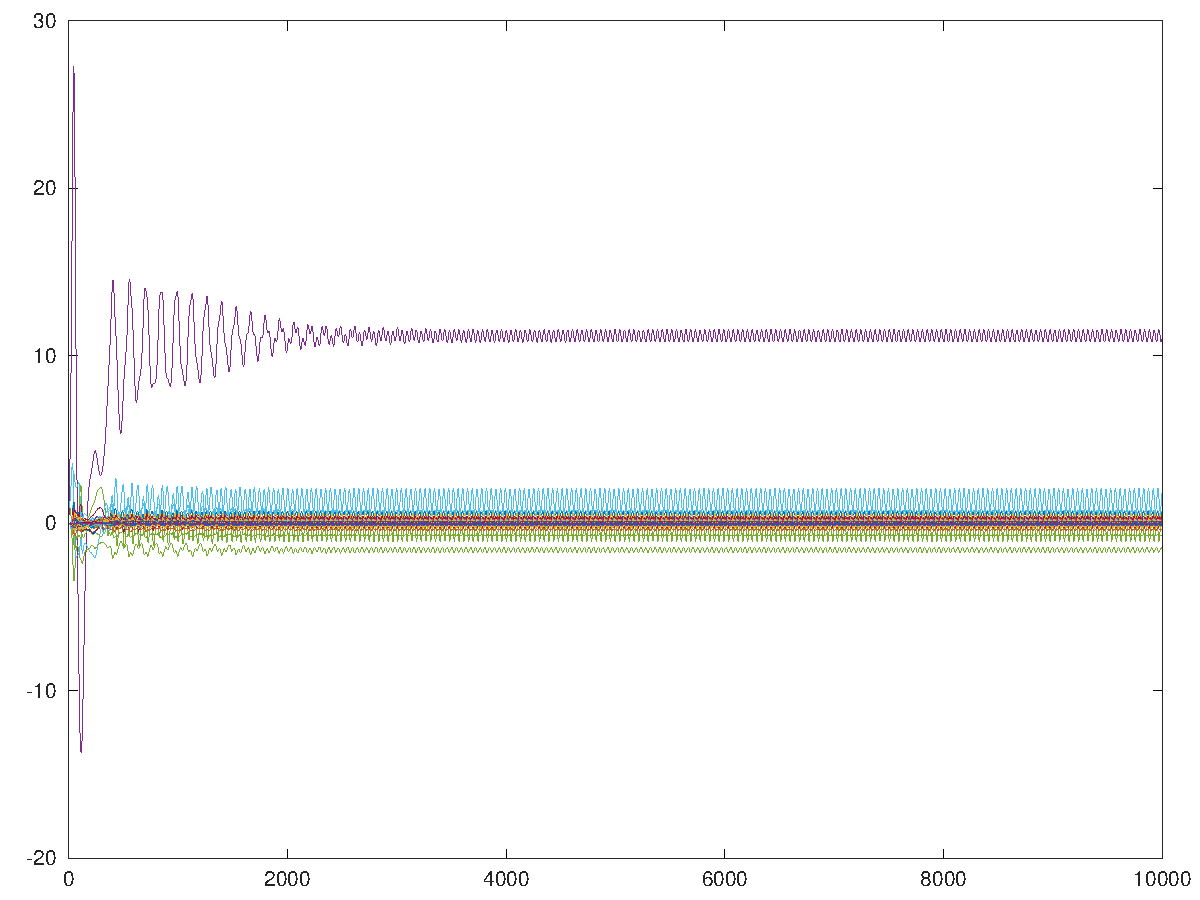
\includegraphics[width=0.49\linewidth]{{lorenz2/03-images/ord15.X}.pdf}
	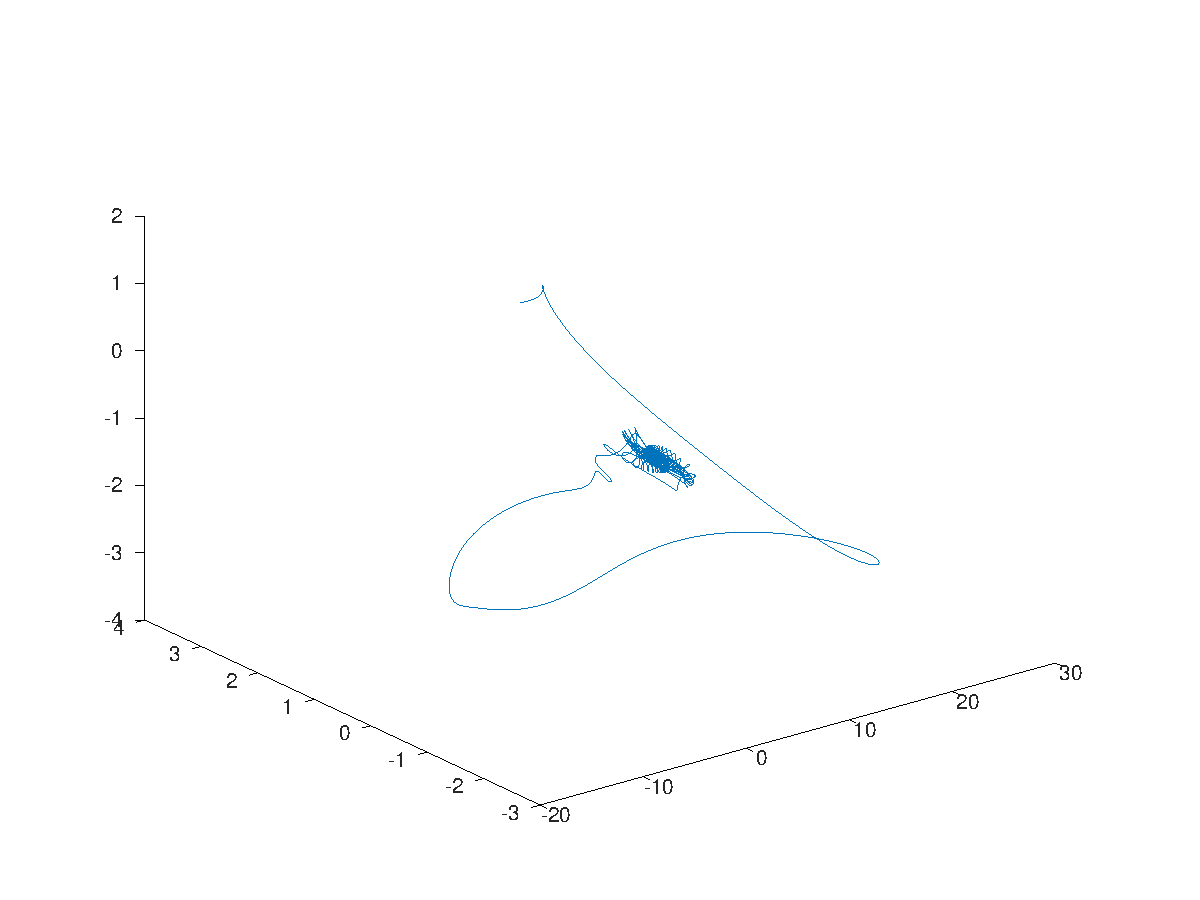
\includegraphics[width=0.49\linewidth]{{lorenz2/03-images/ord15.butterfly}.pdf}
	\caption{Lorenzssystem mit Grad 15, $t = [0,100]$}
	\label{figure:lorenz2:systemdeg15}
\end{figure}

\begin{figure}
	\centering
	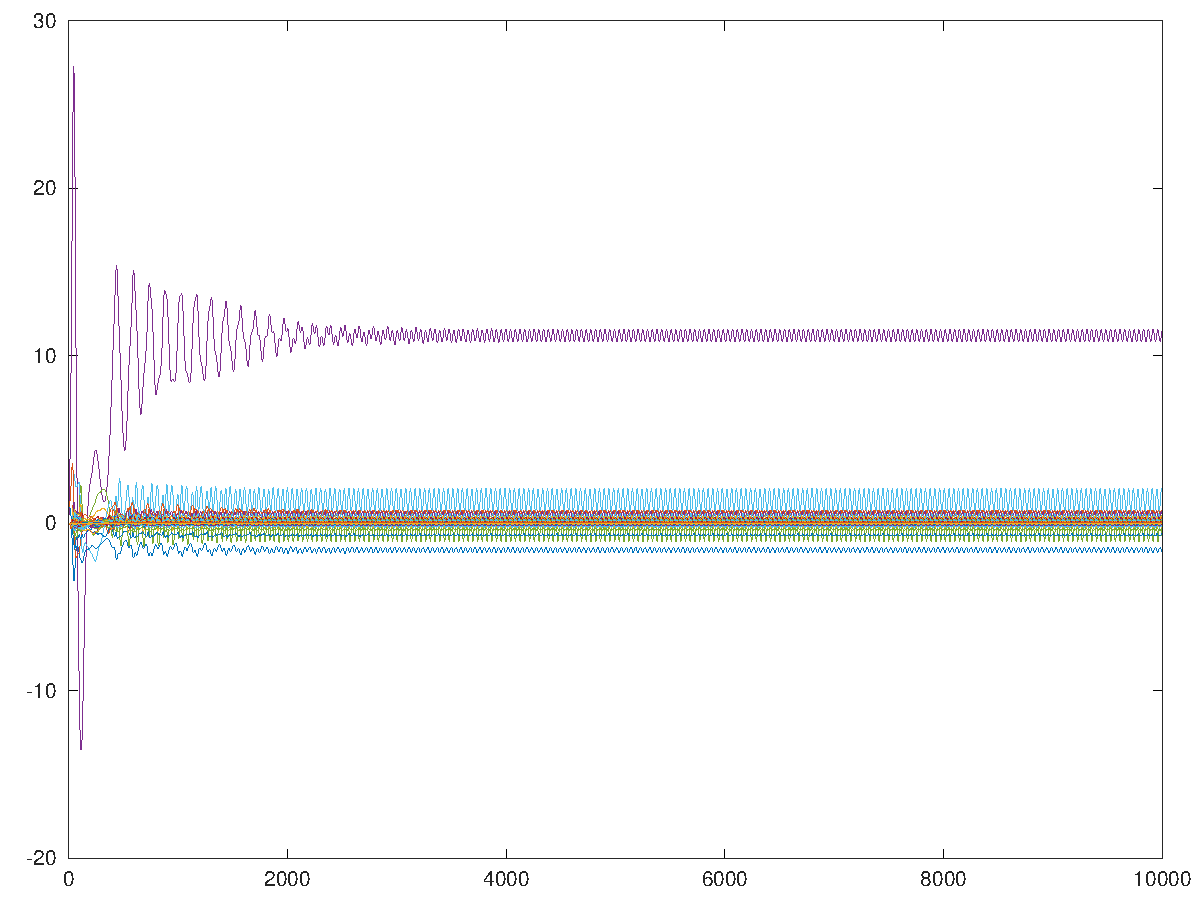
\includegraphics[width=0.49\linewidth]{{lorenz2/03-images/ord16.X}.pdf}
	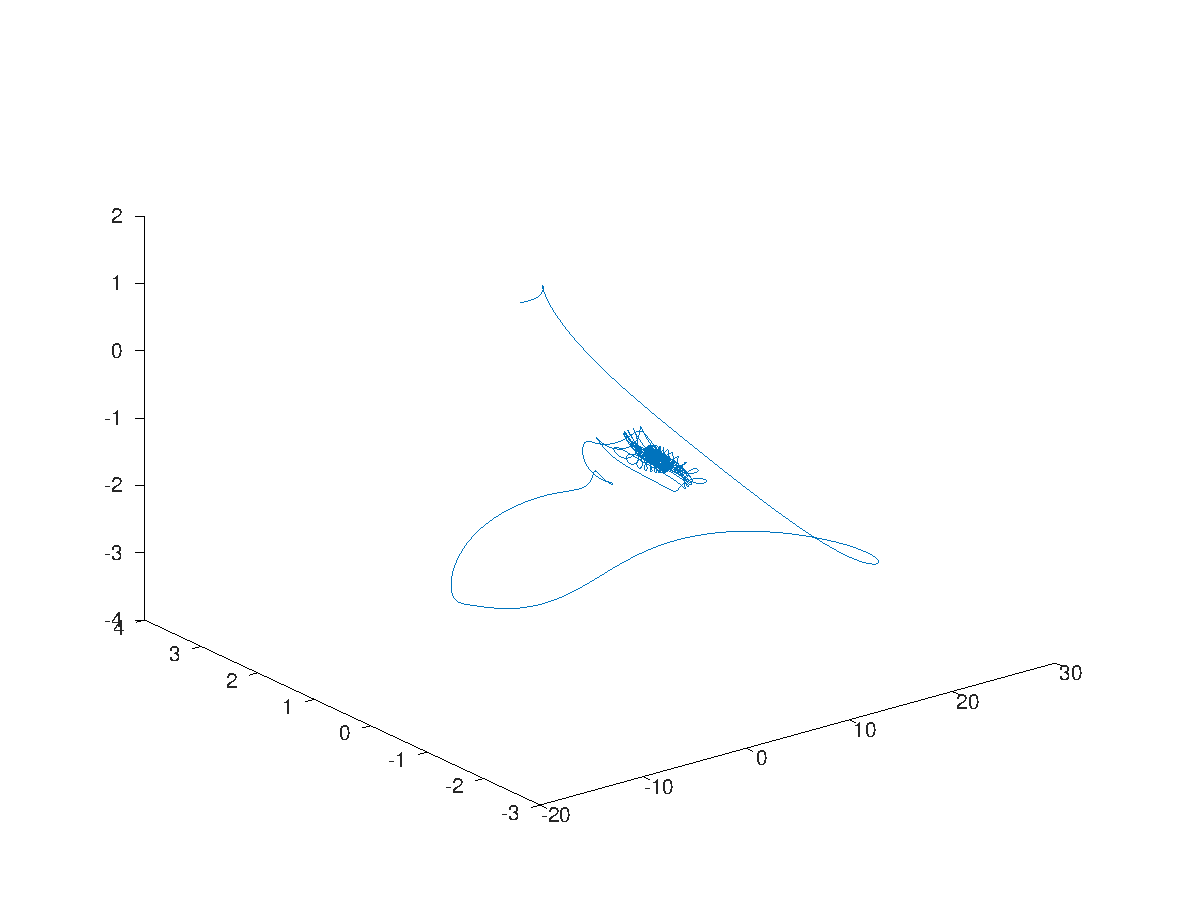
\includegraphics[width=0.49\linewidth]{{lorenz2/03-images/ord16.butterfly}.pdf}
	\caption{Lorenzssystem mit Grad 16, $t = [0,100]$}
	\label{figure:lorenz2:systemdeg16}
\end{figure}

\begin{figure}
	\centering
	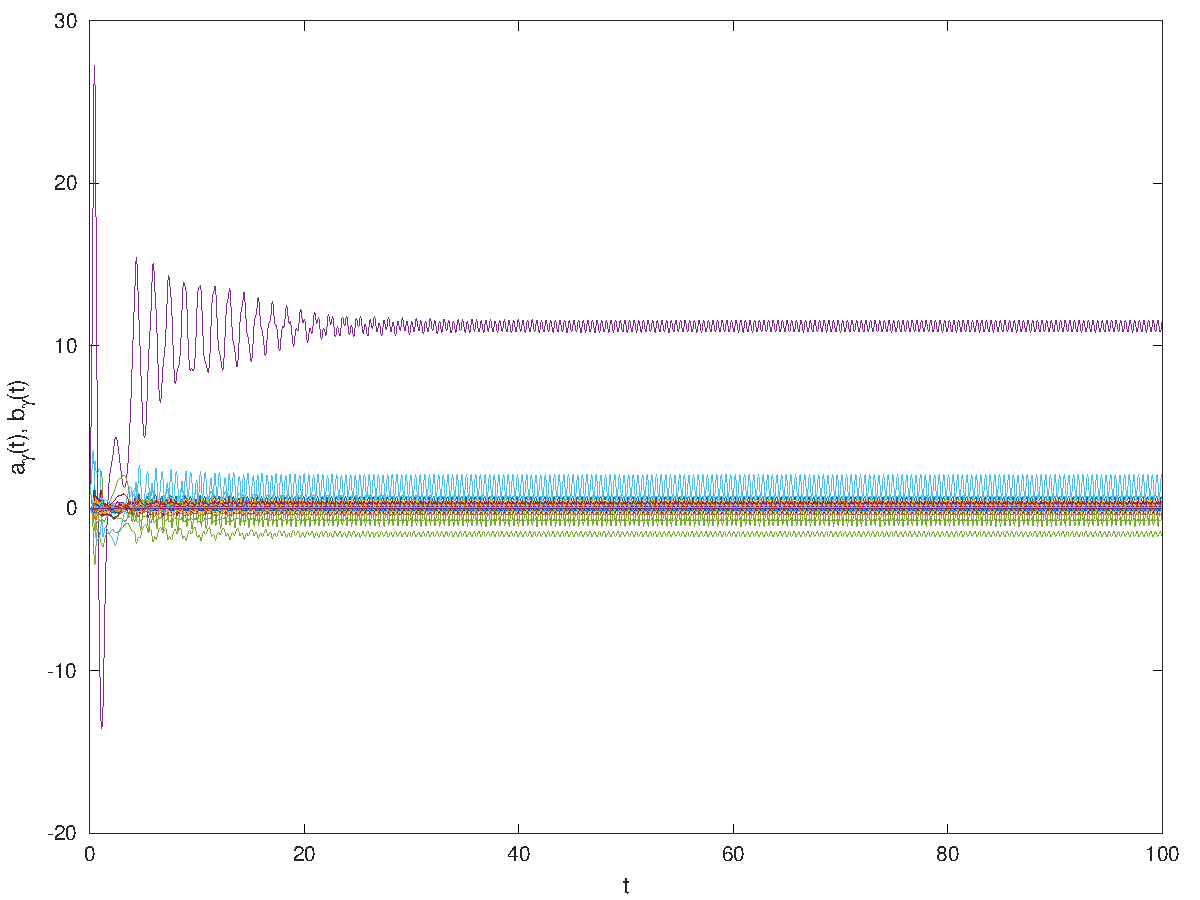
\includegraphics[width=0.49\linewidth]{{lorenz2/03-images/ord17.X}.pdf}
	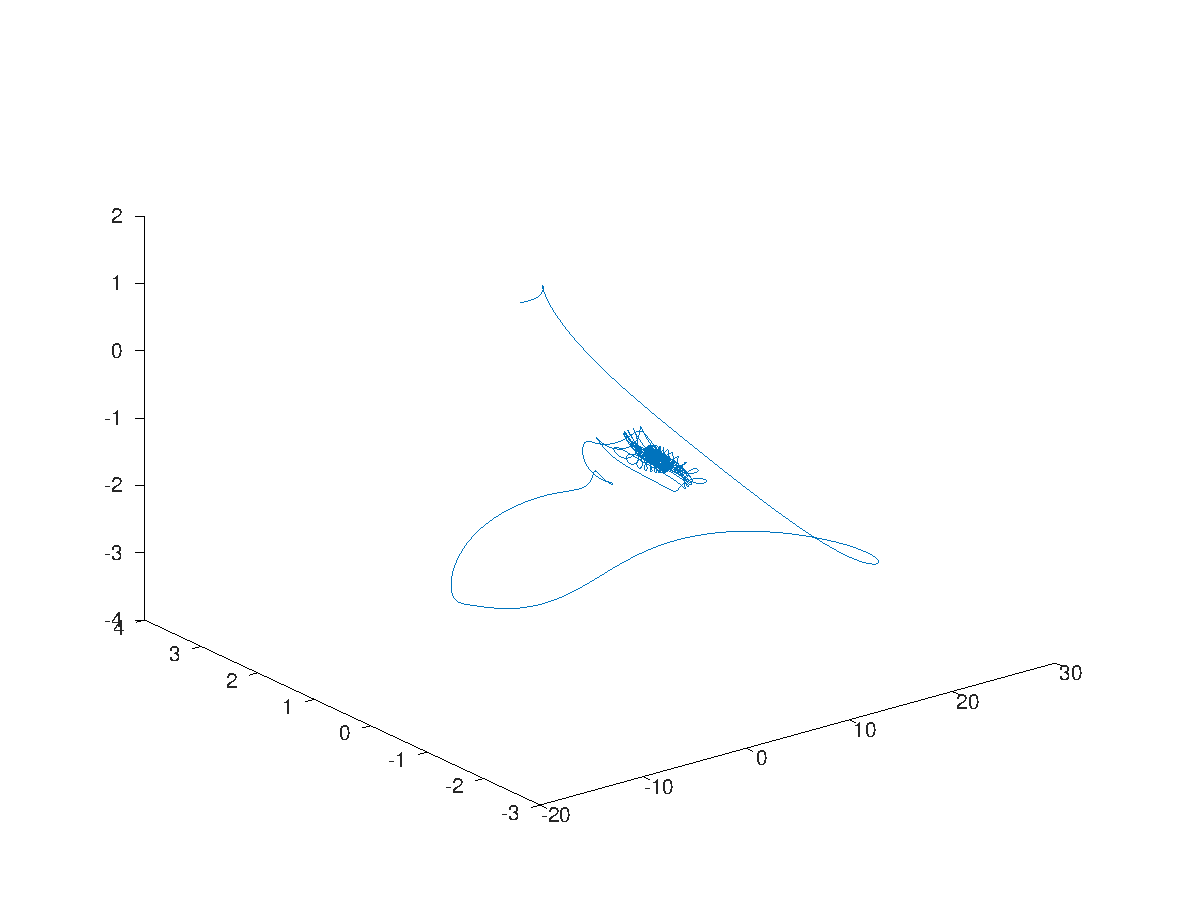
\includegraphics[width=0.49\linewidth]{{lorenz2/03-images/ord17.butterfly}.pdf}
	\caption{Lorenzssystem mit Grad 17, $t = [0,100]$}
	\label{figure:lorenz2:systemdeg17}
\end{figure}

\begin{figure}
	\centering
	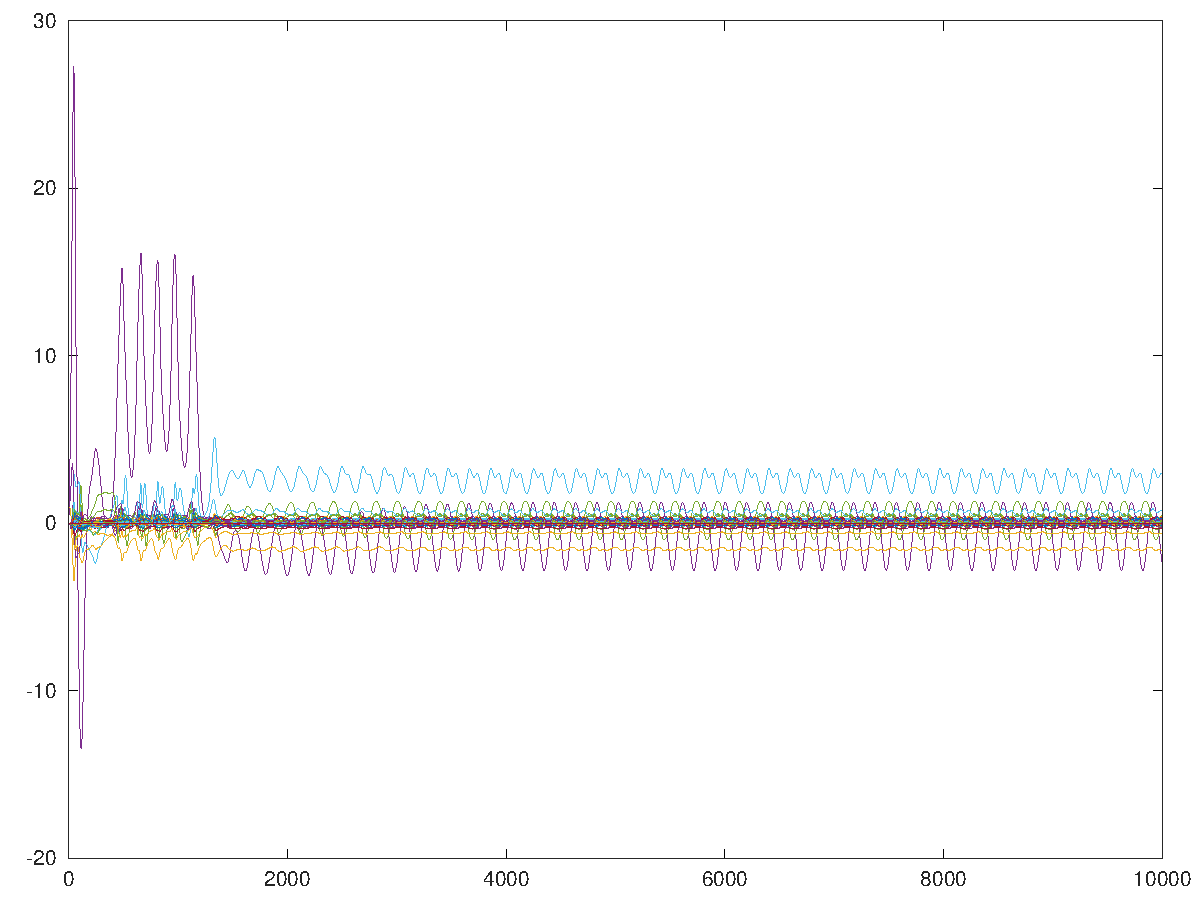
\includegraphics[width=0.49\linewidth]{{lorenz2/03-images/ord18.X}.pdf}
	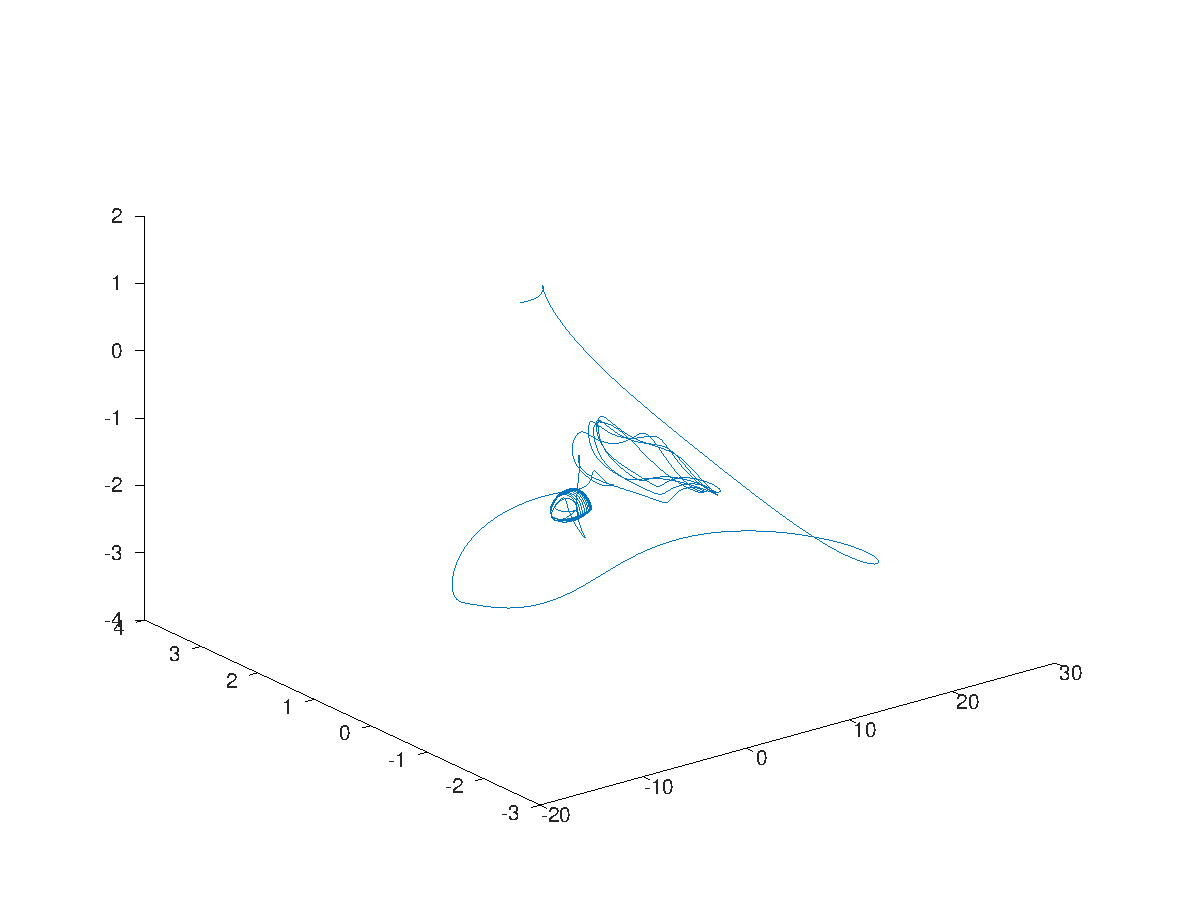
\includegraphics[width=0.49\linewidth]{{lorenz2/03-images/ord18.butterfly}.pdf}
	\caption{Lorenzssystem mit Grad 18, $t = [0,100]$}
	\label{figure:lorenz2:systemdeg18}
\end{figure}

\begin{figure}
	\centering
	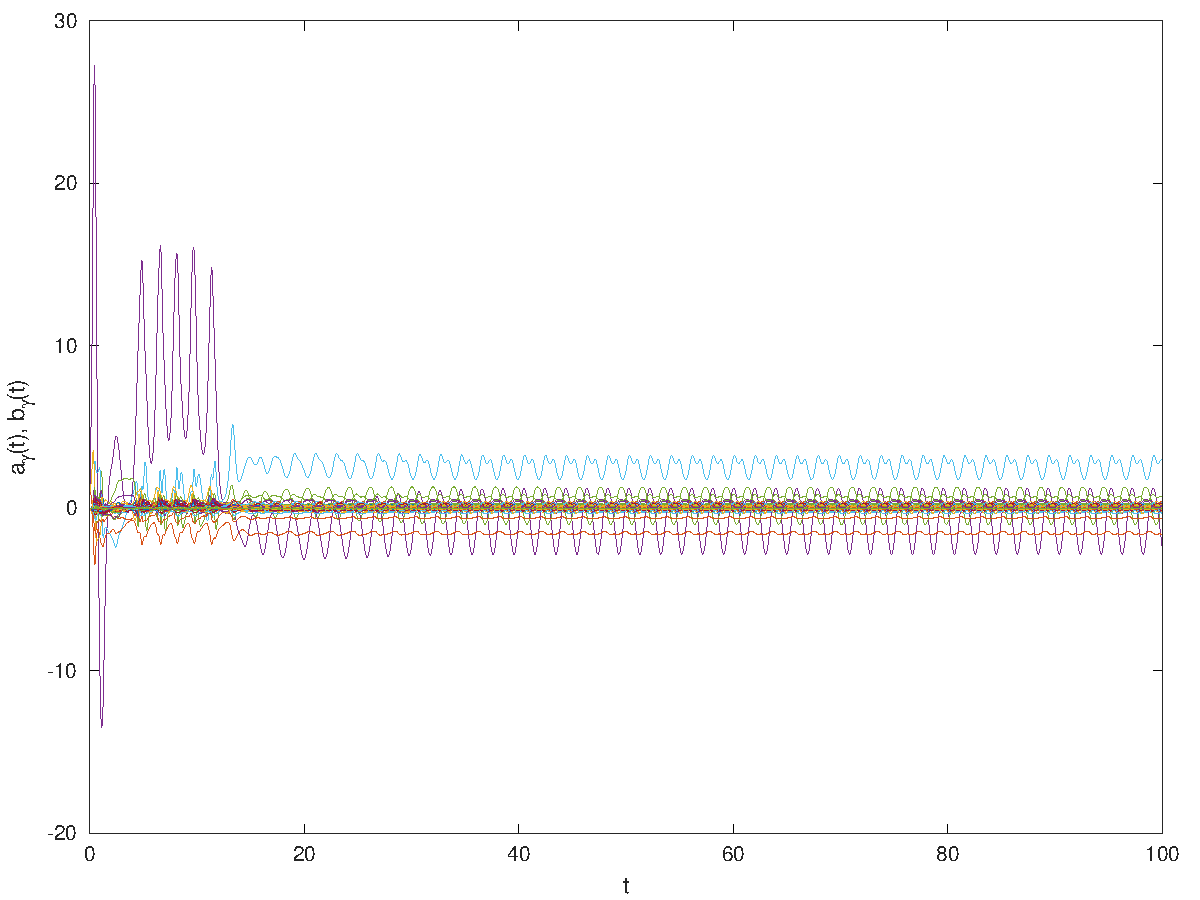
\includegraphics[width=0.49\linewidth]{{lorenz2/03-images/ord19.X}.pdf}
	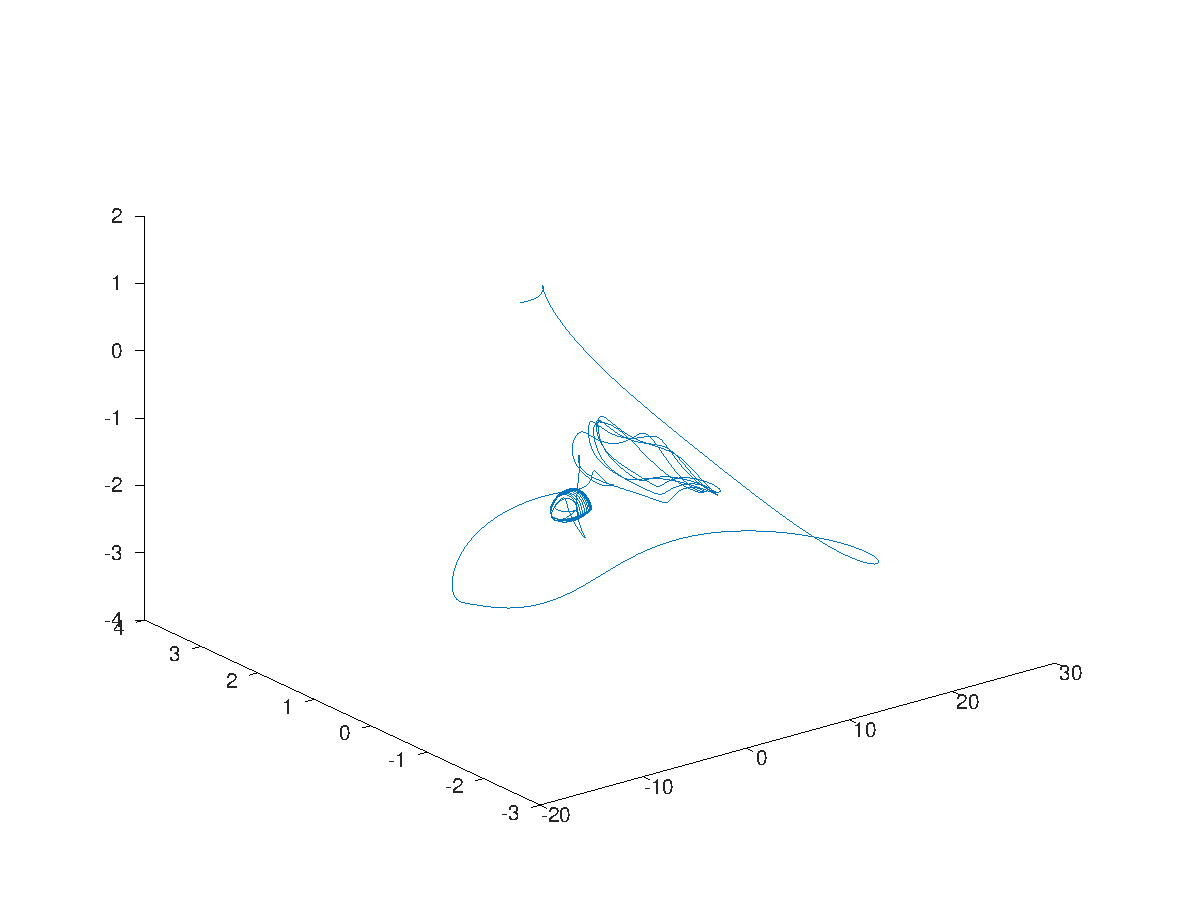
\includegraphics[width=0.49\linewidth]{{lorenz2/03-images/ord19.butterfly}.pdf}
	\caption{Lorenzssystem mit Grad 19, $t = [0,100]$}
	\label{figure:lorenz2:systemdeg19}
\end{figure}

\begin{figure}
	\centering
	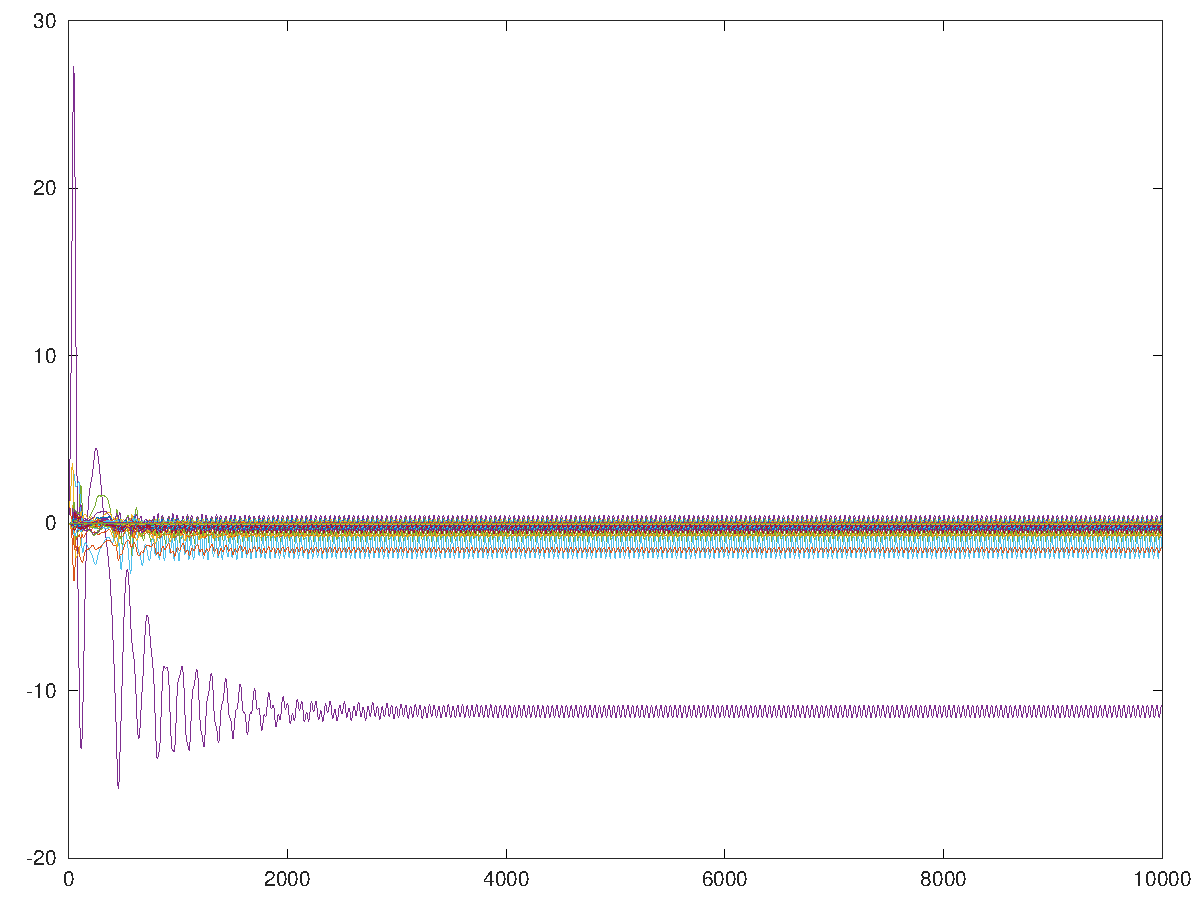
\includegraphics[width=0.49\linewidth]{{lorenz2/03-images/ord20.X}.pdf}
	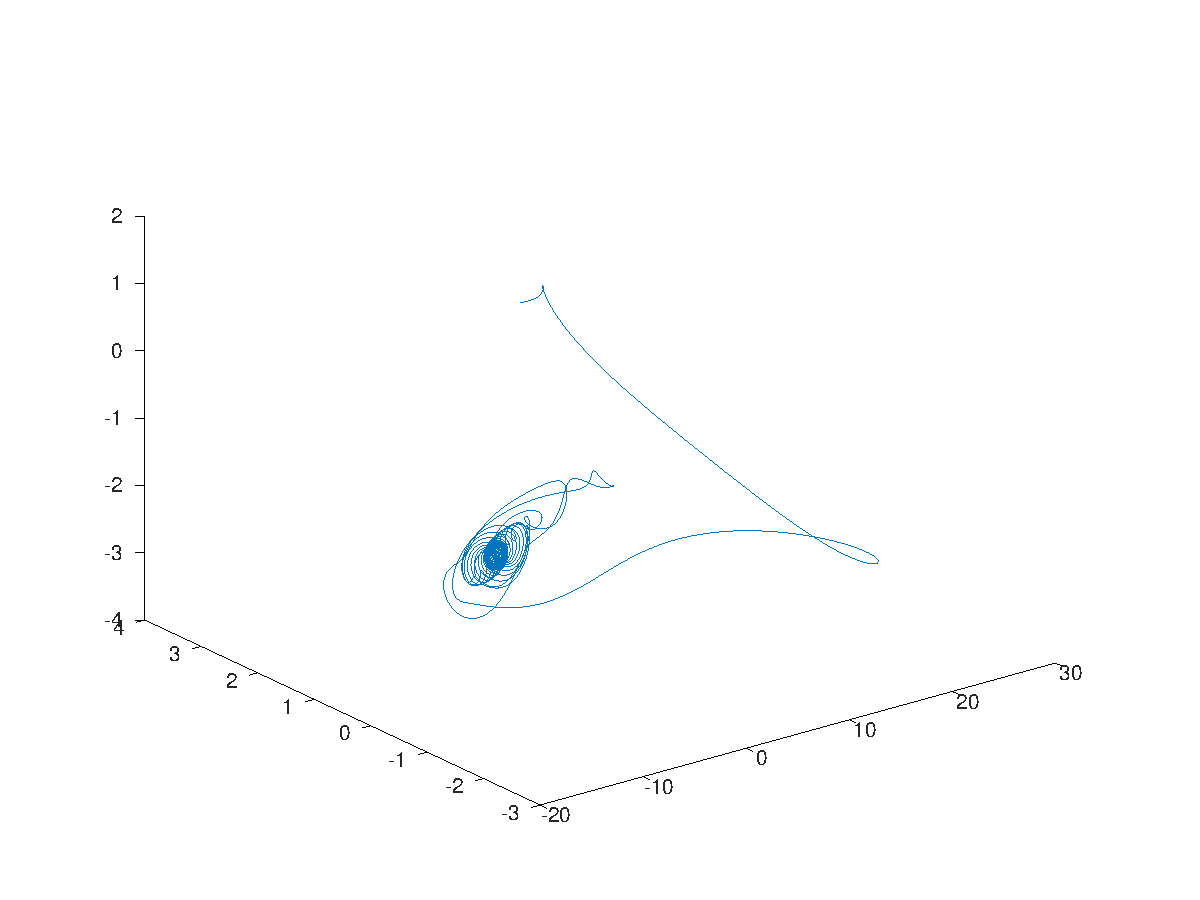
\includegraphics[width=0.49\linewidth]{{lorenz2/03-images/ord20.butterfly}.pdf}
	\caption{Lorenzssystem mit Grad 20, $t = [0,100]$}
	\label{figure:lorenz2:systemdeg20}
\end{figure}

\begin{figure}
	\centering
	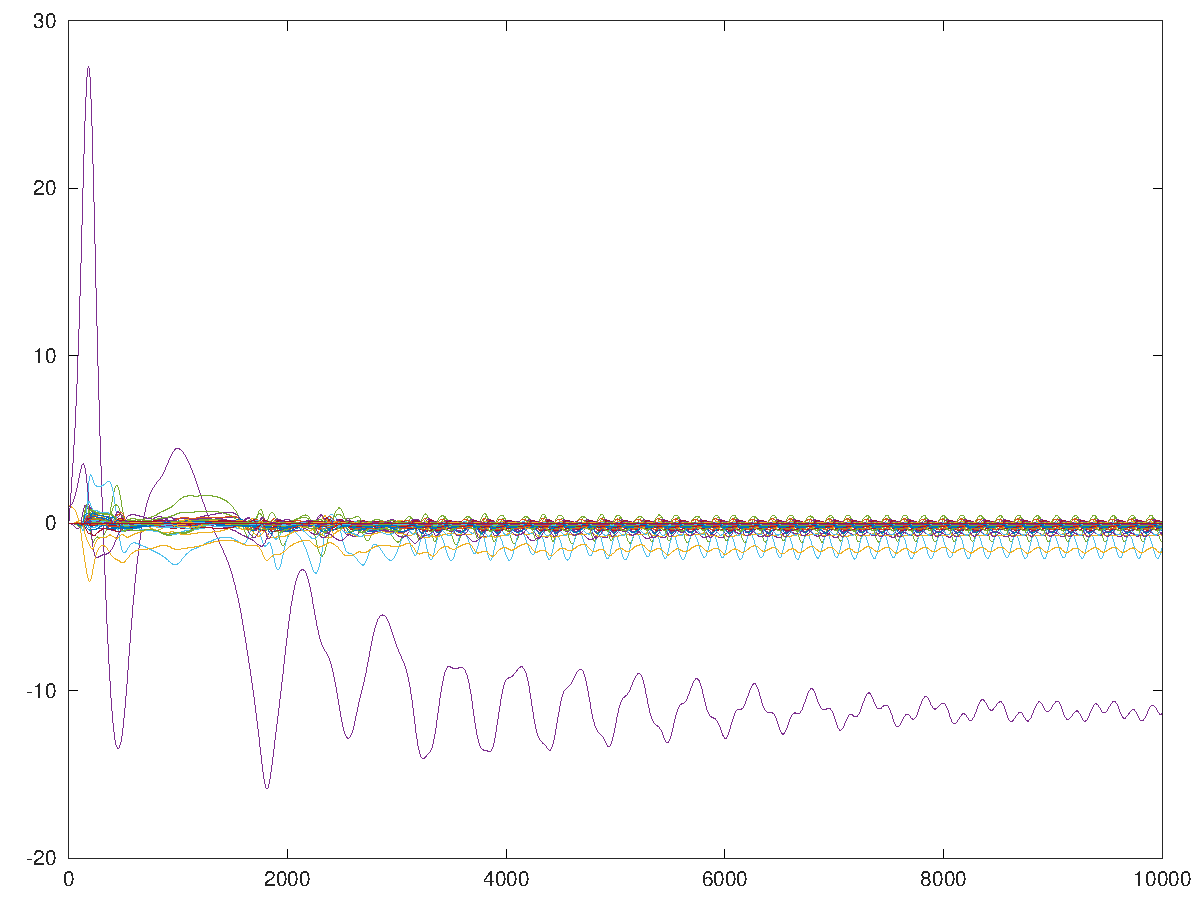
\includegraphics[width=0.49\linewidth]{{lorenz2/03-images/ord21.X.40}.pdf}
	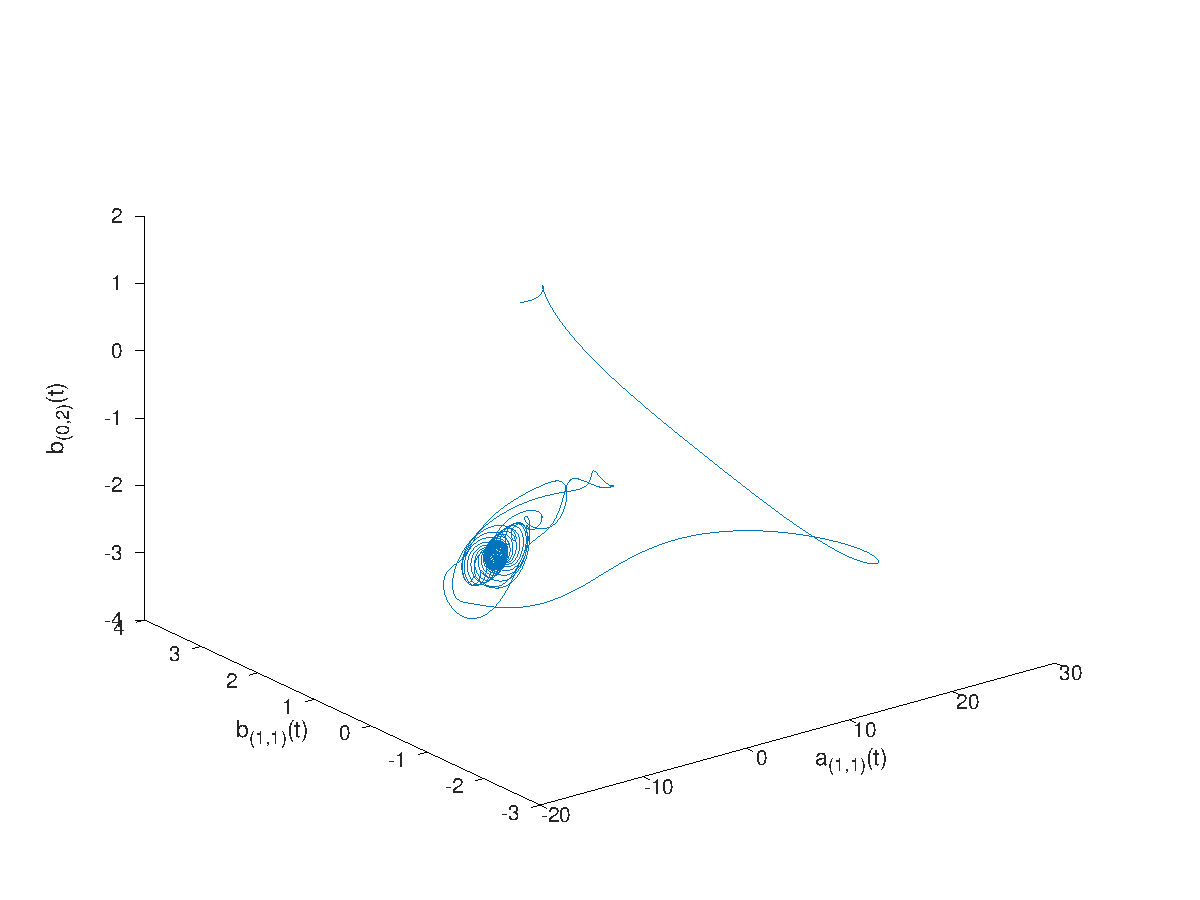
\includegraphics[width=0.49\linewidth]{{lorenz2/03-images/ord21.butterfly.40}.pdf}
	\caption{Lorenzssystem mit Grad 21, $t = [0,40]$}
	\label{figure:lorenz2:systemdeg21-40}
\end{figure}

\begin{figure}
	\centering
	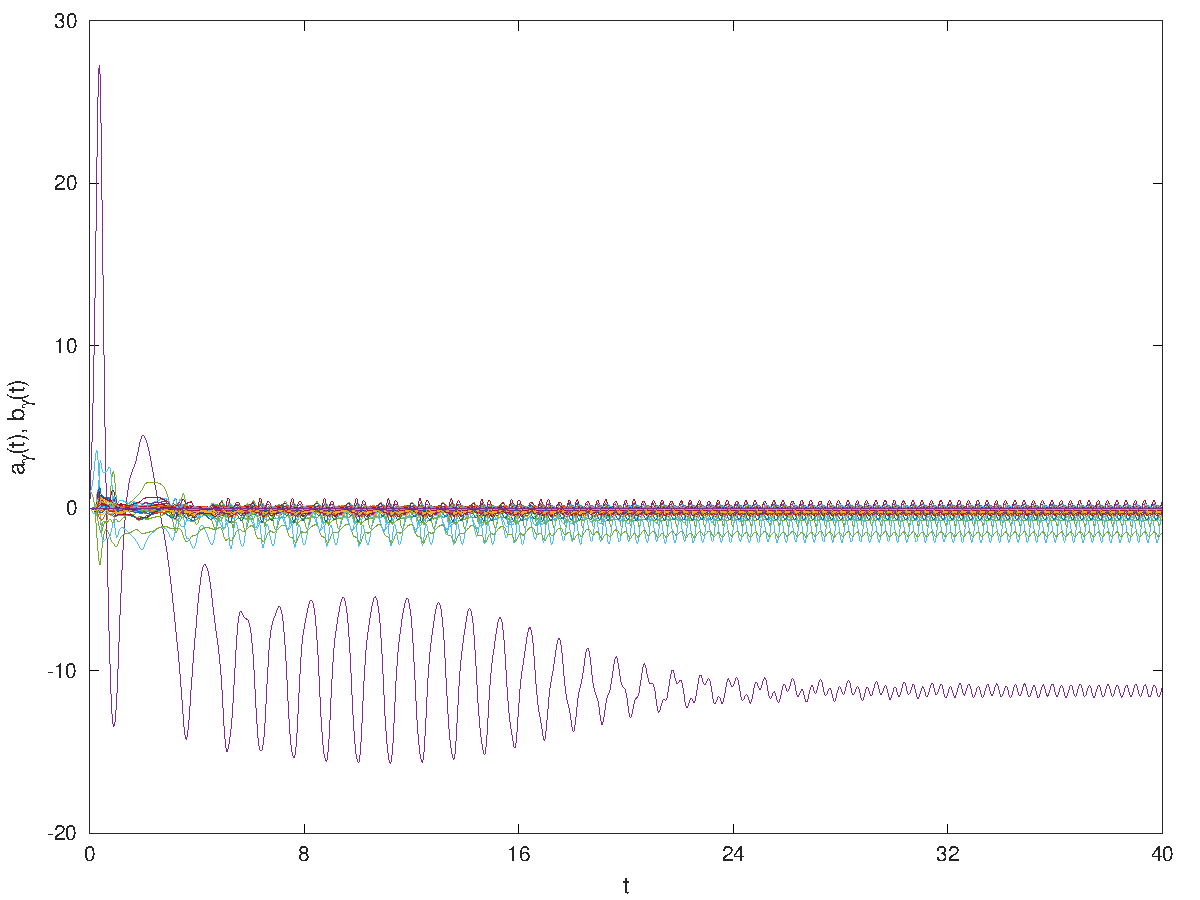
\includegraphics[width=0.49\linewidth]{{lorenz2/03-images/ord22.X.40}.pdf}
	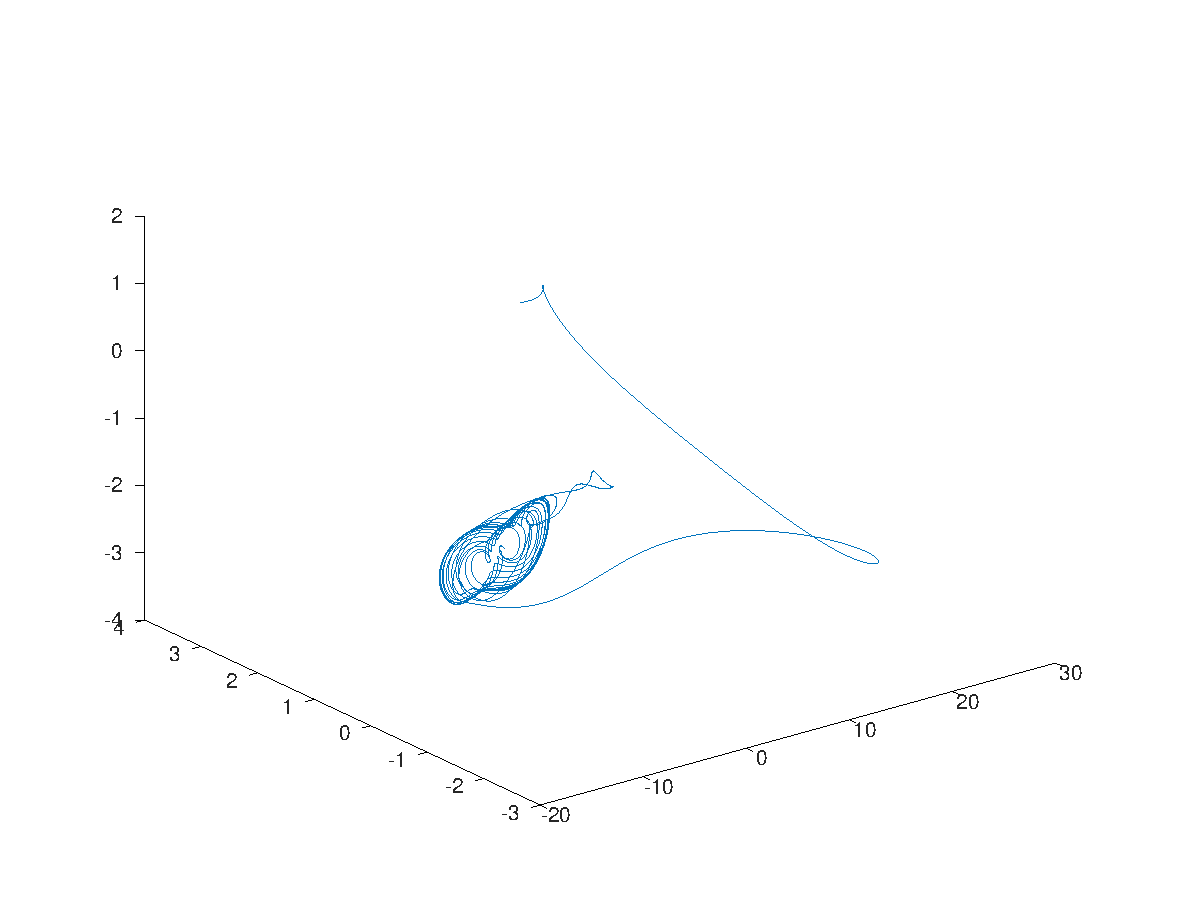
\includegraphics[width=0.49\linewidth]{{lorenz2/03-images/ord22.butterfly.40}.pdf}
	\caption{Lorenzssystem mit Grad 22, $t = [0,40]$}
	\label{figure:lorenz2:systemdeg22-40}
\end{figure}
